\newcommand{\verfasser}{Phil Steinhorst}					% Verfasser des Dokuments
\newcommand{\fach}{Elliptische Kurven und Kryptographie}				% Titel der Vorlesung								
\newcommand{\shortFach}{EKK}								% Titel kurz
\newcommand{\prof}{PD Dr. Karin Halupczok}					% Dozent
\newcommand{\untertitel}{gelesen von \prof}					% Untertitel
\newcommand{\semester}{Sommersemester 2015}					% Semester
\newcommand{\homepage}{http://wwwmath.uni-muenster.de/u/karin.halupczok/ellKKSoSe15/}	% Vorlesungshomepage
% % % % % % % % % % % % % % % % % % % % % % % % % % % % % % % % %
%		PhistScript.tex											%
%		XeLaTeX-Konfiguration für Skripte						%
%																%
%		Author: Phil Steinhorst									%
% % % % % % % % % % % % % % % % % % % % % % % % % % % % % % % % %

\RequirePackage[thinlines]{easybmat} %-- muss aufgrund eines Bugs vor etex und tikz geladen werden
\documentclass[a4paper, twoside, headsepline, index=totoc,toc=listof, fontsize=9pt, cleardoublepage=empty, headinclude, DIV=13, BCOR=13mm, titlepage]{scrartcl}

\usepackage{scrtime} 	% KOMA, Uhrzeit ermoeglicht
\usepackage{scrpage2} 	% wie fancyhdr, nur optimiert auf KOMA-Skript, leicht andere Syntax
\usepackage{etoolbox}

\usepackage[usenames, table, x11names]{xcolor}	% Farben. Vor TikZ laden!

% % % TikZ-Pakete % % %
\usepackage{tikz}
\usepackage{tikz-cd}
\usetikzlibrary{external}
\tikzset{>=latex}
\usetikzlibrary{shapes,arrows,intersections}
\usetikzlibrary{calc,3d}
\usetikzlibrary{decorations.pathreplacing,decorations.markings}
\usetikzlibrary{angles}
\tikzexternalize[prefix=tikz/, up to date check=diff]	% -shell-escape-Flag nötig!

% % % verwende LuaLaTeX, wegen dynamischer Speicherallokation
\tikzset{external/system call={xelatex \tikzexternalcheckshellescape 
    -halt-on-error -interaction=batchmode -jobname "\image" "\texsource"}}
    
% % % tikzexternalize für tikzcd deaktivieren, da inkompatibel
\AtBeginEnvironment{tikzcd}{\tikzexternaldisable}
\AtEndEnvironment{tikzcd}{\tikzexternalenable}

% % % um Inkompatibilitaeten von quotes und polyglossia bzw. babel zu vermeiden
\tikzset{
  every picture/.append style={
    execute at begin picture={\shorthandoff{"}},
    execute at end picture={\shorthandon{"}}
  }
}
\usetikzlibrary{quotes}
\usepackage{pgfplots}

% % % Mathe-Zeugs
\usepackage{mathtools} 						% beinhaltet amsmath
\mathtoolsset{showonlyrefs, centercolon}
\usepackage{wasysym}
\usepackage{amssymb} 						% zusätzliche Symbole
\usepackage{latexsym} 						% zusätzliche Symbole
\usepackage{stmaryrd} 						% für Blitz
\usepackage{nicefrac} 						% schräge Brüche
\usepackage{cancel} 						% Befehle zum Durchstreichen
\usepackage{extarrows}						% mehr Pfeile
\usepackage{mathdots}
\DeclareSymbolFont{bbold}{U}{bbold}{m}{n}
\DeclareSymbolFontAlphabet{\mathbbold}{bbold}
\newcommand{\mathds}[1]{\mathbb{#1}} 		% um Kompatibilitaet mit frueheren Benutzung von dsfont herzustellen
\def\mathul#1#2{\color{#1}\underline{{\color{black}#2}}\color{black}} %farbiges Untersteichen im Mathe-Modus

% % % XeTeX & Fonts
\usepackage{mathspec} 						% beinhaltet fontspec 
\usepackage{polyglossia} 					% babel-Ersatz
\setmainlanguage[spelling=new,babelshorthands=false]{german}
\newcommand\glqq{"}
\newcommand\grqq{"}
\defaultfontfeatures{Mapping=tex-text, WordSpace={1.4}} %
\setmainfont[Ligatures=Common, BoldFont={* Bold}, ItalicFont={* Light Italic}]{Source Sans Pro}
\setsansfont[Scale=MatchLowercase,Ligatures=Common, BoldFont={* Medium}]{Ubuntu}
\setallmonofonts[Scale=MatchLowercase, ItalicFont={*}]{Consolas} 
\usepackage{xltxtra}
\usepackage{fontawesome}

% % % Misc.
\usepackage[neverdecrease]{paralist}
\usepackage[german=quotes]{csquotes}
\usepackage{booktabs}
\usepackage{wrapfig}
\usepackage{float}
\usepackage[margin=10pt, font=small, labelfont=sf, format=plain, indention=1em]{caption}
\captionsetup[wrapfigure]{name=Abb. }
\usepackage{stackrel}
\usepackage{ifthen}
\usepackage{multicol}
%\flushbottom

% % % Unterstreichung
\usepackage[normalem]{ulem}
\setlength{\ULdepth}{1.8pt}

% % % Indexverarbeitung
\usepackage{makeidx}
\newcommand{\bet}[1]{\textbf{#1}}
\newcommand{\Index}[1]{\textbf{#1}\index{#1}}
\makeindex
\renewcommand{\indexpagestyle}{scrheadings}

% % % Marginnote & todonotes
\usepackage{marginnote}
\renewcommand*{\marginfont}{\color{gray} \footnotesize }
\usepackage[textsize=small]{todonotes}
\makeatletter
\renewcommand{\todo}[2][]{\tikzexternaldisable\@todo[#1]{#2}\tikzexternalenable}
\makeatother

% % % Konfiguration von Hyperref pdfstartview=FitH, 
\usepackage[hidelinks, pdfpagelabels,  bookmarksopen=true, bookmarksnumbered=true, linkcolor=black, urlcolor=RoyalBlue3, plainpages=false, hypertexnames=false, citecolor=black, hypertexnames=true, pdfauthor={\verfasser}, pdfborderstyle={/S/U}, linkbordercolor=RoyalBlue3, colorlinks=true, unicode, pdfencoding=auto]{hyperref}

\newcommand{\RM}[1]{\MakeUppercase{\romannumeral #1{}}} 	% Römische Zahlen
\usepackage{ellipsis}										% Punkte

% % % % % % % % % % % % % % % % % % % % % % % % % % % % % % % % %
%		PhistMath.tex											%
%		Weitere Mathe-Befehle									%
%																%
%		Author: Phil Steinhorst									%
% % % % % % % % % % % % % % % % % % % % % % % % % % % % % % % % %

% % % Buchstaben und Zahlen
\newcommand{\CC}{\mathbb{C}}
\newcommand{\FF}{\mathbb{F}}
\newcommand{\HH}{\mathbb{H}}
\newcommand{\KK}{\mathbb{K}}
\newcommand{\NN}{\mathbb{N}}
\newcommand{\OO}{\mathbb{O}}
\newcommand{\QQ}{\mathbb{Q}}
\newcommand{\RR}{\mathbb{R}}
\newcommand{\ZZ}{\mathbb{Z}}
\newcommand{\bigO}{\mathcal{O}}					% Landau-O
\newcommand{\ind}{1\hspace{-0,9ex}1} 			% Indikatorfunktion (Doppeleins)

% % % Abk�rzungen
\newcommand{\ab}[1]{\overline{#1}}					% Abschluss
\newcommand{\bewrueck}{\glqq$\Leftarrow$\grqq:} 	% Beweis R�ckrichtung
\newcommand{\bewhin}{\glqq$\Rightarrow$\grqq:}		% Beweis Hinrichtung
\newcommand{\borel}{\mathfrak{B}}					% Borelsche Sigma-Algebra
\newcommand{\setone}{\{1\}}							% Einsmenge
\newcommand{\leb}{\lambda \hspace{-0,95ex}\lambda}	% Lebesgue-Ma� (Doppel-Lambda)
\newcommand{\Lp}{\mathcal{L}}						% L^p-R�ume
\newcommand{\NT}{\trianglelefteq}					% Normalteiler
\newcommand{\setnull}{\{0\}}						% Nullmenge
\newcommand{\weak}{\rightharpoonup}					% schwache Konvergenz
\newcommand{\weaks}{\overset{*}{\rightharpoonup}}	% schwache *-Konvergenz
\newcommand{\salg}{\mathfrak{A}}					% Sigma-Algebra (Skript-A)
\newcommand{\zyklot}[1]{#1^{(\infty)}}				% zyklotomische Erweiterung


% % % Operatoren
\DeclareMathOperator{\Alt}{Alt} 					% Alternierende n-Linearform
\DeclareMathOperator{\Aut}{Aut} 					% Automorphismen
\DeclareMathOperator{\Bil}{Bil} 					% Bilinearformen
\DeclareMathOperator{\bild}{Bild} 					% Bild
\DeclareMathOperator{\dom}{dom} 					% Domain
\DeclareMathOperator{\diam}{diam}					% Durchmesser
\DeclareMathOperator{\dist}{dist} 					% Distanz
\DeclareMathOperator{\eqs}{\mathrel{\widehat{=}}}	% entspricht
\DeclareMathOperator{\diver}{div} 					% Gradient
\DeclareMathOperator{\EPK}{EPK} 					% Einpunktkompaktifizierung
\DeclareMathOperator{\End}{End} 					% Endomorphismen
\DeclareMathOperator{\esssup}{esssup}				% essentielles Supremum
\DeclareMathOperator{\Gal}{Gal}	 					% Galoisgruppe
\DeclareMathOperator{\ggT}{ggT} 					% ggT
\DeclareMathOperator{\GL}{GL}						% allgemeine lineare Gruppe
\DeclareMathOperator{\grad}{grad} 					% Gradient
\DeclareMathOperator{\Grad}{Grad} 					% Grad
\DeclareMathOperator{\Hess}{Hess} 					% Hesse-Matrix
\DeclareMathOperator{\Hom}{Hom} 					% Homomorphismen
\DeclareMathOperator{\id}{id} 						% identische Abbildung
\DeclareMathOperator{\im}{im} 						% image
\DeclareMathOperator{\Jac}{Jac} 					% Jacobson-Radikal
\DeclareMathOperator{\Kern}{Kern}					% Kern
\DeclareMathOperator{\kgV}{kgV} 					% kgV
\DeclareMathOperator{\Koker}{Koker} 				% Kokern
\DeclareMathOperator{\Cov}{Cov} 					% Kovarianz
\DeclareMathOperator{\Mod}{Mod} 					% Moduln
\DeclareMathOperator{\modu}{mod} 					% Modulo
\DeclareMathOperator{\ord}{ord} 					% Ordnung
\DeclareMathOperator{\der}{\partial}				% Partielle Ableitung
\DeclareMathOperator{\pot}{\mathcal{P}}				% Potenzmenge
\DeclareMathOperator{\prlim}{\varprojlim\limits}	% projektiver Limes
\DeclareMathOperator{\Quot}{Quot}					% Quotientenring
\DeclareMathOperator{\Rang}{Rang} 					% Rang
\DeclareMathOperator{\rot}{rot} 					% Rotation
\DeclareMathOperator{\sgn}{sgn} 					% Signum
\DeclareMathOperator{\Spec}{Spec} 					% Spektrum
\DeclareMathOperator{\SL}{SL} 						% Spezielle lineare Gruppe
\DeclareMathOperator{\SO}{SO} 						% Spezielle orthogonale Gruppe
\DeclareMathOperator{\SU}{SU} 						% Spezielle unit�re Gruppe
\DeclareMathOperator{\Spur}{Spur} 					% Spur
\DeclareMathOperator{\supp}{supp} 					% Tr�ger
\DeclareMathOperator{\Sym}{Sym} 					% Symmetrische Gruppe
\DeclareMathOperator{\tr}{tr} 						% trace

% % % Klammerungen
\DeclarePairedDelimiter{\abs}{\lvert}{\rvert}		% Betrag
\DeclarePairedDelimiter{\ceil}{\lceil}{\rceil}		% aufrunden
\DeclarePairedDelimiter{\floor}{\lfloor}{\rfloor}	% aufrunden
\DeclarePairedDelimiter{\sprod}{\langle}{\right}	% spitze Klammern
\DeclarePairedDelimiter{\enbrace}{(}{)}				% runde Klammern
\DeclarePairedDelimiter{\benbrace}{[}{]}			% eckige Klammern
\DeclarePairedDelimiter{\penbrace}{\{}{\}}			% geschweifte Klammern

% % % Norm
\DeclarePairedDelimiter\doppelstrich{\Vert}{\Vert}
\newcommand{\norm}[2][\relax]{
\ifx#1\relax \ensuremath{\doppelstrich*{#2}}
\else \ensuremath{\doppelstrich*{#2}_{#1}}
\fi}							% selbst definierte Mathe-Befehle

\setlength\parindent{0pt}             % ohne Einrueckung

% % % Konfiguration von scrheadings
\setheadsepline{1pt}[\color{black}]
\pagestyle{scrheadings}
\clearscrheadfoot

% % % Kopf-/Fußzeilenlayout
\providecommand{\shortFach}{\fach}
\ohead{\small \leftmark}
\ofoot[{ \small \thepage}]{ \small \thepage} 
\automark{section}

% Metadaten
\title{\fach}
\author{\verfasser}
\subtitle{\untertitel}
\date{\semester}

% Inhaltsverzeichnis
\usepackage[tocindentauto]{tocstyle}
\usetocstyle{KOMAlike}	

% ntheorem package
\usepackage[hyperref]{ntheorem}			% Lade ntheorem mit hyperref-Workaround
\theoremstyle{break}					% Zeilenumbruch nach Theoremkopf
\theorembodyfont{\normalfont}			% nicht kursiv
\theorempreskipamount0.5cm				% Abstand vor Theorem
\theorempostskipamount0.5cm				% Abstand nach Theorem

% Workaround für Tabulatoren im Theorem-Verzeichnis
\makeatletter
\def\thm@@thmline@name#1#2#3#4{%
        \@dottedtocline{-2}{0em}{2.3em}%
                   {\makebox[\widesttheorem][l]{#1 \protect\numberline{#2}}#3}%
                   {#4}}
\@ifpackageloaded{hyperref}{
\def\thm@@thmline@name#1#2#3#4#5{%
    \ifx\\#5\\%
        \@dottedtocline{-2}{0em}{2.3em}%
            {\makebox[\widesttheorem][l]{#1 \protect\numberline{#2}}#3}%
            {#4}
    \else
        \ifHy@linktocpage\relax\relax
            \@dottedtocline{-2}{0em}{2.3em}%
                {\makebox[\widesttheorem][l]{#1 \protect\numberline{#2}}#3}%
                {\hyper@linkstart{link}{#5}{#4}\hyper@linkend}%
        \else
            \@dottedtocline{-2}{0em}{2.3em}%
                {\hyper@linkstart{link}{#5}%
                  {\makebox[\widesttheorem][l]{#1 \protect\numberline{#2}}#3}\hyper@linkend}%
                    {#4}%
        \fi
    \fi}
}
\makeatother
\newlength\widesttheorem
\AtBeginDocument{
  \settowidth{\widesttheorem}{Proposition 10.10\quad}	% Referenzstring für die Breite der ersten Spalte
}

\theoremlisttype{optname}	% nur Theoreme auflisten, die einen Namen haben. 

\newcommand{\qed}{\ifmmode \tag*{$\square$} \else \hfill $\square$ \fi} % qed-Symbol.							% XeLaTeX-Konfiguration für Skripte

% % % Dokumentspezifische Einstellungen % % %
\setcounter{tocdepth}{3}				% Tiefe im Inhaltsverzeichnis (1: nur Sections, 2: auch subsections...)

\numberwithin{equation}{section}			% Section in Equation-Nummerierung einbeziehen
\newcounter{counter}						% Zähler für Sätze
\newcounter{lecture}
\numberwithin{counter}{lecture}		% Section in Satz-Nummerierung einbeziehen

\newcommand{\nextlecture}{\stepcounter{lecture} \setcounter{counter}{0}}

% ab hier können neue Umgebungen für Sätze definiert und benannt werden!
% Syntax: \newtheorem{interner Umgebungsname}[Zähler]{Name im Dokument}
% Möchte man Sätze und Definitionen getrennt durchnummerieren, benötigt man weitere Zähler.
\newtheorem{satz}[counter]{Satz}
\newtheorem{defn}[counter]{Definition}
\newtheorem{bem}[counter]{Bemerkung}
\newtheorem{bsp}[counter]{Beispiel}
\newtheorem{lemma}[counter]{Lemma}
\newtheorem{folg}[counter]{Folgerung}
\newtheorem{zusatz}[counter]{Zusatz}
\newtheorem{anw}[counter]{Anwendung}
\newtheorem{erl}[counter]{Erläuterung}
\newtheorem{mot}[counter]{Motivation}
% % % % % % % % % % % % % % % % % % % % % % %
\newcommand{\PP}{\mathbb{P}}
\DeclareMathOperator{\li}{li}
\newcommand{\kon}{\equiv}
\newcommand{\oh}{\mathcal{O}}

% % % % % % % % % % % % % % % % % % % % % % %
\begin{document}
% % % % % % % % % % % % % % % % % % % % % % % % % % % % % % % % %
%		PhistTitle.tex											%
%		Layout für Skript-Titelseiten							%
%																%
%		Author: Phil Steinhorst									%
% % % % % % % % % % % % % % % % % % % % % % % % % % % % % % % % %
\begin{titlepage}
\pagestyle{empty}
\begin{center}
\begin{minipage}{0.4\textwidth}
\begin{flushleft}

\includegraphics[height=1.5cm,keepaspectratio]{../!config/wwulogo.pdf}
\end{flushleft}
\end{minipage}
\hfill
\begin{minipage}{0.4\textwidth}
\begin{flushright}
\vspace*{0.3cm}

\includegraphics[height=1.2cm,keepaspectratio]{../!config/fb10logo.pdf} \
\end{flushright}
\end{minipage}

% Title
\vspace*{2cm}
\textbf{\Huge{\fach}} \\
\vspace{0.2cm} 
\textbf{{\LARGE \untertitel}} \\
\vspace{0.6cm}
\LARGE{Zusammenfassung von \verfasser} \\
\vspace{0.6cm}
\LARGE{\semester} \\
\vspace*{1.5cm}
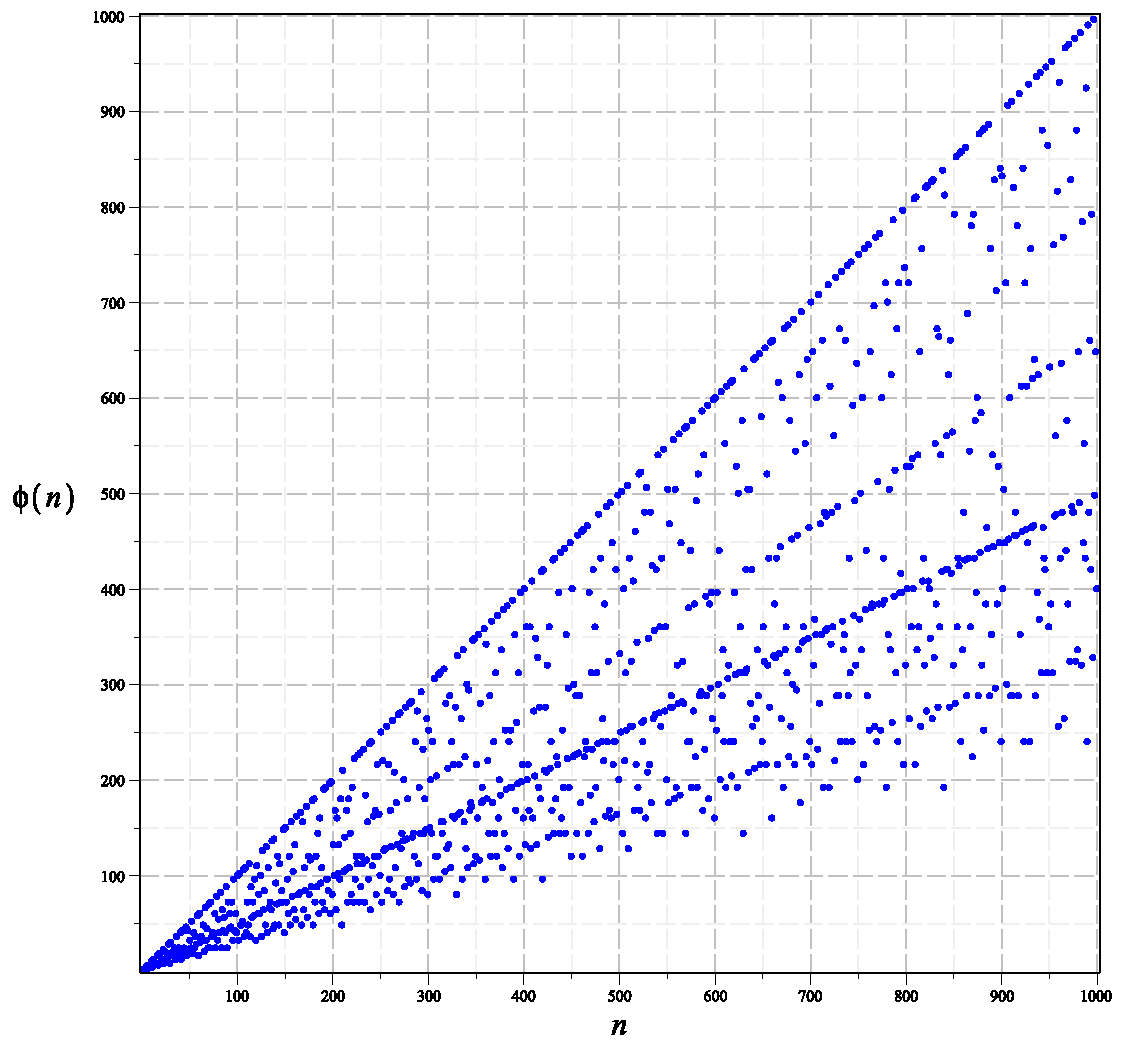
\includegraphics[width=10cm,keepaspectratio]{content/totient.pdf} \\
\vspace*{1cm}
\footnotesize{\url{\homepage}} \\

\vfill
\vspace*{1.5cm}
\begin{flushright}
{\footnotesize Stand: \today}
\end{flushright}
\end{center}
\end{titlepage}							% Titelseite ausgeben
\section*{Vorwort}
\label{sec:preface}
	Der vorliegende Text ist eine Zusammenfassung zur Vorlesung Elementare Zahlentheorie, gelesen von Prof. Dr. Falko Lorenz an der WWU Münster im Wintersemester 2014/2015. Der Inhalt entspricht weitestgehend dem Skript, welches auf der Vorlesungswebsite bereitsgestellt wird, jedoch wird auf Beweise weitestgehend verzichtet. Dieses Werk ist keine Eigenleistung des Autors und wird nicht vom Dozenten der Veranstaltung korrekturgelesen. Für die Korrektheit des Inhalts wird daher keinerlei Garantie übernommen. Bemerkungen, Korrekturen und Ergänzungen kann man folgenderweise loswerden:
	\begin{itemize}
		\item persönlich durch Überreichen von Notizen oder per E-Mail
		\item durch Abändern der entsprechenden TeX-Dateien und Versand per E-Mail an mich
		\item direktes Mitarbeiten via GitHub. Dieses Skript befindet sich im \texttt{latex-wwu}-Repository von Jannes Bantje:
		\begin{center}
			\url{https://github.com/JaMeZ-B/latex-wwu}
		\end{center}
	\end{itemize}

\subsection*{Literatur}
\label{sub:lit}
\begin{itemize}
	\item F. Ischebeck: \href{http://wwwmath.uni-muenster.de/u/ischebeck/}{Einladung zur Zahlentheorie}
	\item R. Remmert, P. Ullrich: \href{http://link.springer.com/book/10.1007/978-3-7643-7731-1}{Elementare Zahlentheorie}
	\item A. Scholz, B. Schöneberg: Einführung in die Zahlentheorie
	\item K. Halupczok: \href{http://wwwmath.uni-muenster.de/u/karin.halupczok/ElZthSS2009Skript.pdf}{Skript zur Elementaren Zahlentheorie}
\end{itemize}

\subsection*{Vorlesungswebsite}
\label{sub:link}
Das vollständige Skript des Dozenten sowie weiteres Material findet man unter folgendem Link:
\begin{center}
	\url{\homepage}
\end{center}

\subsection*{Titelbild}
\label{sub:titlepic}
Plot der Eulerschen $\varphi$-Funktion für $1 \leq n \leq 1000$, erstellt mit Maple. Zugehöriges Maple-Worksheet befindet sich im Git-Repository (siehe oben).

\vfill
\begin{flushright}
	Phil Steinhorst \\
	p.st@wwu.de
\end{flushright}
\newpage
\tableofcontents
\newpage											% Inhaltsverzeichnis ausgeben
\setcounter{section}{-1}
\section{Motivation und Einführung}
\label{sec:para0}

\nextlecture
\subsection*{Kryptologie}
	Die \textbf{Kryptologie} besteht aus den folgenden beiden Gebieten: \marginnote{[1]} 
	\begin{description}
		\item[Kryptographie:] Studium mathematischer Techniken zur Verschlüsselung von Informationen oder geheimen Nachrichten und dem Schutz von Daten.
		\item[Kryptoanalyse:] Beschreibung der Rückgewinnung von Informationen aus verschlüsselten Texten, der Entschlüsselung.
	\end{description}
Oft meint man mit "Kryptographie" die Kryptologie. \\

Früher wurde die Kryptographie vor allem im militärischen oder diplomatischen Sektor verwendet, heutzutage steht in unserer vernetzten Welt vor allem auch der praktische Nutzen im Alltag im Vordergrund: im Internet einkaufen, Online-Banking, persönliche Daten geheimhalten bzw. Datenschutz, Nachrichten und Dokumente digital unterschreiben etc. Das Internet liefert schnelle Informationswege über öffentliche Kanäle, die leicht abgehört werden können, sodass die Verschlüsselung schützenswerter Daten unumgänglich wird. Auch die Möglichkeit zur Signierung wird nötig, weil sehr leicht Absenderangaben gefälscht werden können. Eventuell nicht abhörsichere Kanäle können außer dem Internet aber auch Briefe, Radio, Boten, etc. sein. \\

Bei der \textbf{symmetrischen Verschlüsselung} von Daten gibt es einen Sender $S$ und einen Empfänger $E$, die sich beide auf einen gemeinsamen Schlüssel geeinigt haben, der zum Ver- und Entschlüsseln dient. Beim \Index{Caesar-Code} z.B. ist dies die Vereinbarung, jeden Buchstaben durch den dritten nachfolgenden im Alphabet zu ersetzen, also $A \mapsto D, B \mapsto E, C \mapsto F$, usw. Die Entschlüsselung ist klar. Derartige \textbf{monoalphabetische Chiffrierungen}, bei der jeder Buchstabe des Alphabets stets durch denselben Geheimtextbuchstaben chiffriert wird, sind durch Häufigkeitsanalysen durch einen Angreifer, der die verschlüsselten Nachrichten abhört, sehr leicht zu entschlüsseln. Übrigens gibt es auch heutzutage PDF-Verschlüsselungsprogramme, die so arbeiten! 

In dieser Vorlesung behandeln wir die heutzutage gängigen modernen Methoden, die als sicher gelten. Worauf diese starke Sicherheit beruht, hat mathematische Gründe, die wir besprechen möchten. Vor allem interessiert uns, wie und welche Mathematik in die Kryptologie kommt, sodass wir deren Verfahren verstehen können. \\

Die Anwendungen erfordern die Lösung folgender Probleme bei symmetrischen Verschlüsselungsverfahren:
\begin{itemize}
	\item Schlüsselaustausch über öffentliche Kanäle (\textbf{öffentliche Schlüssel})
	\item Verschlüsselung ohne vorherigen Schlüsselaustausch (mit \textbf{geheimen Schlüsseln}, die nicht versendet werden)
	\item Digitale Signierung und Autentifizierung
\end{itemize}
Dies können \textbf{asymmetrische Verfahren} leisten (auch \textbf{Public Key-Kryptographie} genannt) und gehen zurück auf Ideen von Diffie\footnote{Whitfield Diffie, \url{http://de.wikipedia.org/wiki/Whitfield_Diffie}} und Hellman\footnote{Martin Hellman, \url{http://de.wikipedia.org/wiki/Martin_Hellman}} aus den 70er Jahren: \\

Jeder Nutzer eines Kommunikationskanals hat einen privaten Schlüssel, den er geheim hält und niemand sonst kennt, sowie einen öffentlichen Schlüssel, den jeder einsehen kann. Eine Nachricht wird dann unter Ausnutzung einer Funktion $x \mapsto f(x)$ verschlüsselt, die zwar leicht zu berechnen, aber praktisch nur mit Kenntnis des privaten Schlüssels des rechtmäßigen Empfängers entschlüsselt werden kann. Der Sender der Nachricht wird dafür den öffentlichen Schlüssel des Empfängers zur Verschlüsselung benutzen. Eine derartige Funktion heißt \Index{Einwegfunktion}.

\minisec{Beispiele}
\begin{itemize}
	\item \Index{RSA-Verfahren}: $(p,q) \mapsto p \cdot q$ mit $p,q$ prim.
	\item \Index{ECC-Verfahren}: $x \mapsto mx$ in einer Gruppe auf einer elliptischen Kurve.
\end{itemize}

In einem ersten Teil der Vorlesung stellen wir gängige Verfahren dar, die leicht mit dem Zahlring $\ZZ$ und Strukturen darin realisiert werden können. Dabei werden wir nur einige Hilfsmittel der elementaren Zahlentheorie entwickeln und dafür heranziehen. In einem zweiten Teil studieren wir die Eigenschaften elliptischer Kurven als interessante geometrische und arithmetische Objekte, die sich in der Praxis der Kryptographie als nützlich erwiesen haben. Wir besprechen dann auch die Sicherheit und Implementierung dieser Verfahren und vergleichen sie miteinander.

\subsection*{Elliptische Kurven}
Was sind elliptische Kurven? Jedenfalls sind elliptische Kurven \textbf{keine} Ellipsen. Ellipsen lassen sich durch Gleichungen der Form
\[ \enbrace*{\frac{x}{a}}^2 + \enbrace*{\frac{y}{b}}^2 = 1 \text{ mit } a,b \in \RR \setminus \setnull \]
beschreiben. Durch die Parametrisierung $x(t) = a \cdot \cos(t), y(t) = b \cdot \sin(t)$ ergibt sich für die Bogenlänge der Ellipse ein elliptisches Integral zweiter Art, nämlich
\[ \int_{0}^{2\pi} \sqrt{ \enbrace*{\frac{dx(t)}{dt}}^2 + \enbrace*{\frac{dy(t)}{dt}}^2 } dt = 4 \int_{0}^{2\pi} \sqrt{ a^2 \cos^2(t) + b^2 \cdot \sin^2 (t)} dt \]
Im Allgemeinen lässt sich dies nicht elementar integrieren (außer natürlich, falls $a = b$, d.h. ein Kreis vorliegt). Mit Hilfe von elliptischen Kurven findet man jedoch nicht-elementare Stammfunktionen für diese Integrale\linebreak ($\Rightarrow$ Funktionentheorie). Aufgrund dieses Zusammenhangs haben elliptische Kurven ihren Namen, sie haben ansonsten nichts mit Ellipsen zutun. \\

Was sind nun elliptische Kurven? Es sind "abelsche Varietäten der Dimension 1". Elliptische Kurven sind spezielle algebraische Kurven über einem Körper $k$. Es handelt sich dabei um glatte kubische Kurven, deren definierende algebraische Gleichung sich meist in die Form
\[ E \colon y^2 = x^3 + ax + b \text{ mit } a,b \in k \]
bringen lässt. Als Punktmenge haben wir dafür
\[ E(k) := \{ (x,y) \in k^2 : y^2 = x^3 + ax + b\} \cup \{ \oh \}, \]
die Kurve hängt nur von $a,b$ ab. Die Rolle des zusätzlichen so genannten "unendlich fernen Punkts" $\oh$ werden wir dabei noch näher beleuchten. \\

Zwei typische Beispiele für elliptische Kurven:
\begin{enumerate}[1)]
	\item $E_1\colon y^2 = x^3 + 17$, hier liegen sogar Punkte mit ganzzahligen Koordinaten auf $E_1$, nämlich $(-2,3), (-1,4), (2,5)$. Die Kurve besteht aus einer Zusammenhangskomponente.
	\item $E_2 \colon y^2 = x^3 + ax + b$, wenn $f(x) = x^3 + ax + b$ drei verschiedene Nullstellen hat, z.B. $a = -3, b= -1$. Die Kurve besteht dann aus zwei Zusammenhangskomponenten.
\end{enumerate}

\begin{figure}[h!]
	\centering
	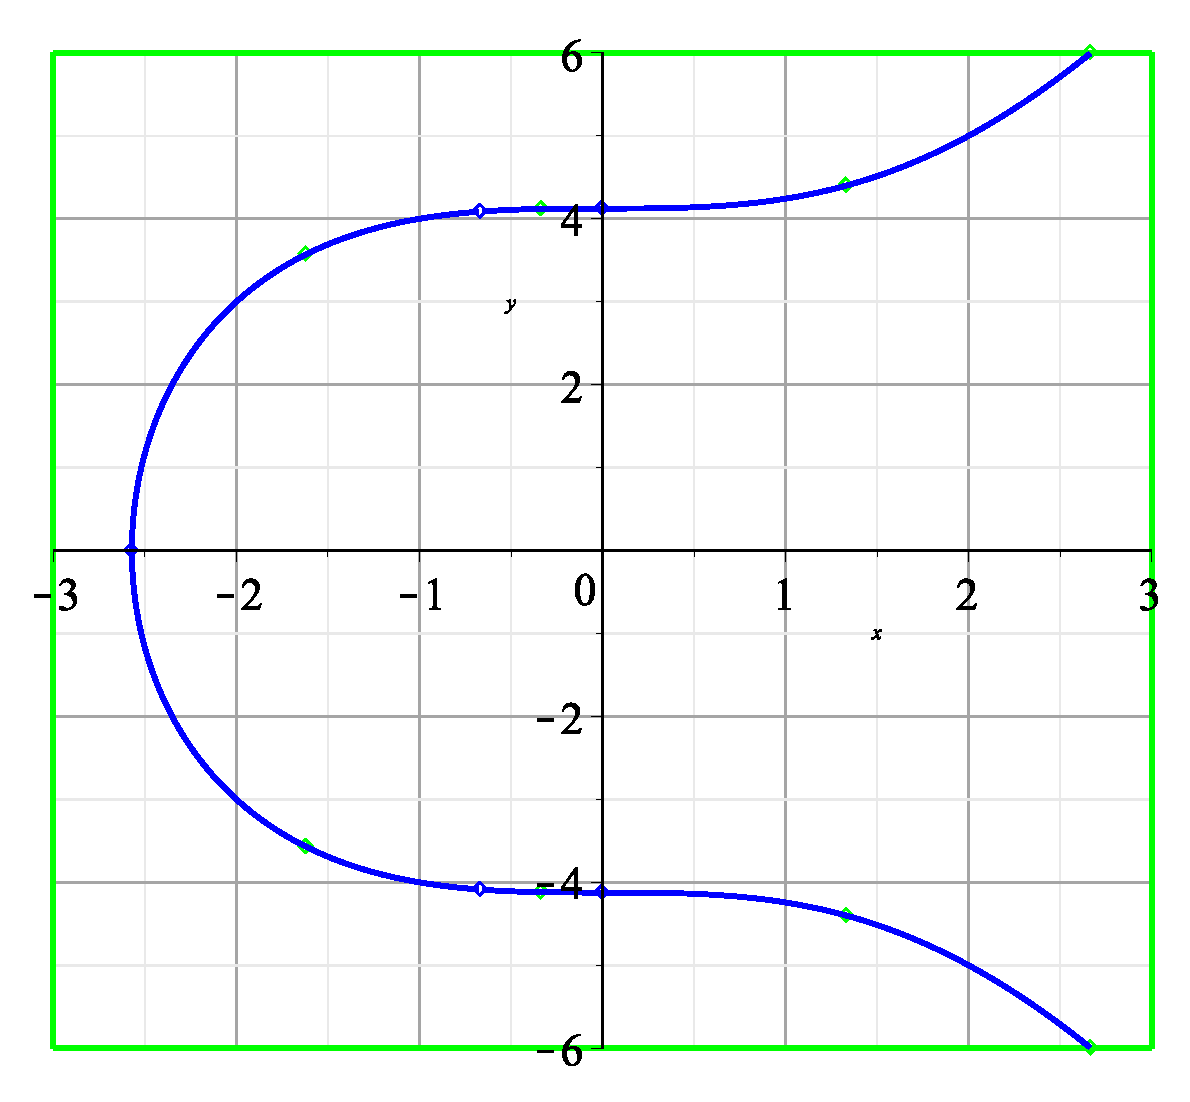
\includegraphics[scale=.3]{img/curve_0_1.eps} \hspace{2cm}
	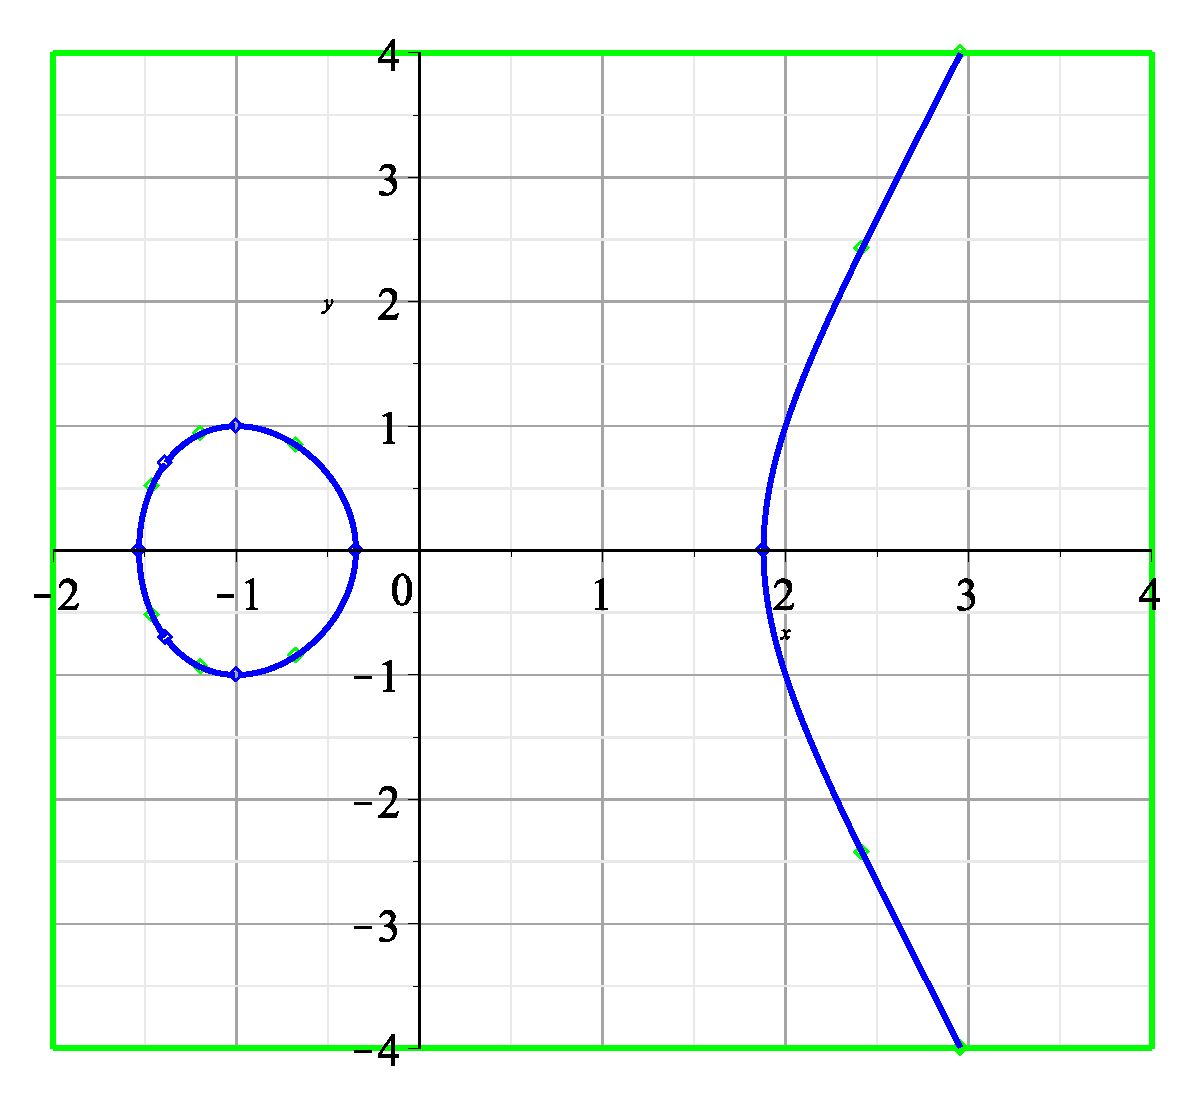
\includegraphics[scale=.3]{img/curve_0_2.eps}
	\caption{Die Kurven $E_1$ (links) und $E_2$ (rechts).}
\end{figure}
%\begin{figure}[h]
%	\centering
%	\begin{tikzpicture}
%	\begin{axis}[
%		scale only axis,
%		xlabel=$x$,
%		ylabel=$y$,
%		grid=major,
%		axis lines=middle,
%		inner axis line style={=>},
%		ymin = -5,
%		ymax = 5,
%		xmin = -3,
%		xmax = 3,
%		xtick={-3,-2,...,3},
%		ytick={-5,-4,...,5}
%	]
%	\addplot[color=red, thick, domain=-2.57128:3, samples=100] {(x^3+17)^(1/2)};
%	\addplot[color=red, thick, domain=-2.57128:3, samples=100] {-(x^3+17)^(1/2)};
%	\end{axis}
%	\end{tikzpicture} \hspace{2cm}
%	\begin{tikzpicture}
%	\begin{axis}[
%		scale only axis,
%		xlabel=$x$,
%		ylabel=$y$,
%		grid=major,
%		axis lines=middle,
%		inner axis line style={=>},
%		ymin = -5,
%		ymax = 5,
%		xmin = -3,
%		xmax = 3,
%		xtick={-3,-2,...,3},
%		ytick={-5,-4,...,5}
%	]
%	\addplot[color=red, thick, domain=-1.53208888:-0.347296, samples=100,unbounded coords=jump] {(x^3-3*x-1)^(1/2)};
%	\end{axis}
%	\end{tikzpicture}
%\end{figure}

\minisec{Bemerkung}
	Die kubischen Kurven $C_1\colon y^2 = x^3 - 3x +2$ und $C_2\colon y^2 = x^3$ z. B. sind jedoch keine elliptischen Kurven, weil diese nicht glatt sind. \\

\begin{figure}[H]
	\centering
	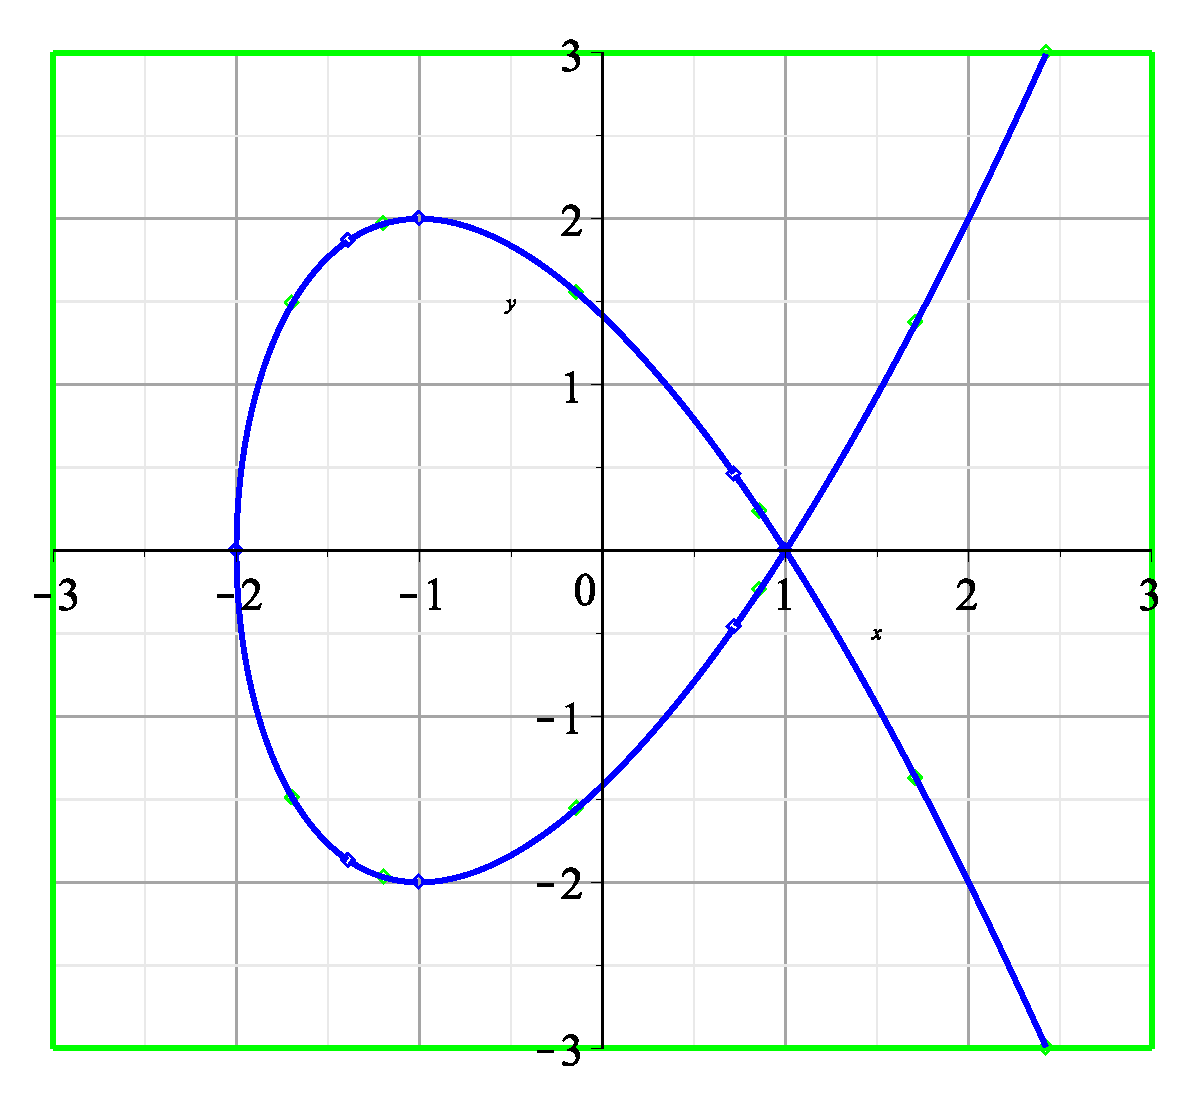
\includegraphics[scale=.3]{img/curve_0_3.eps} \hspace{2cm}
	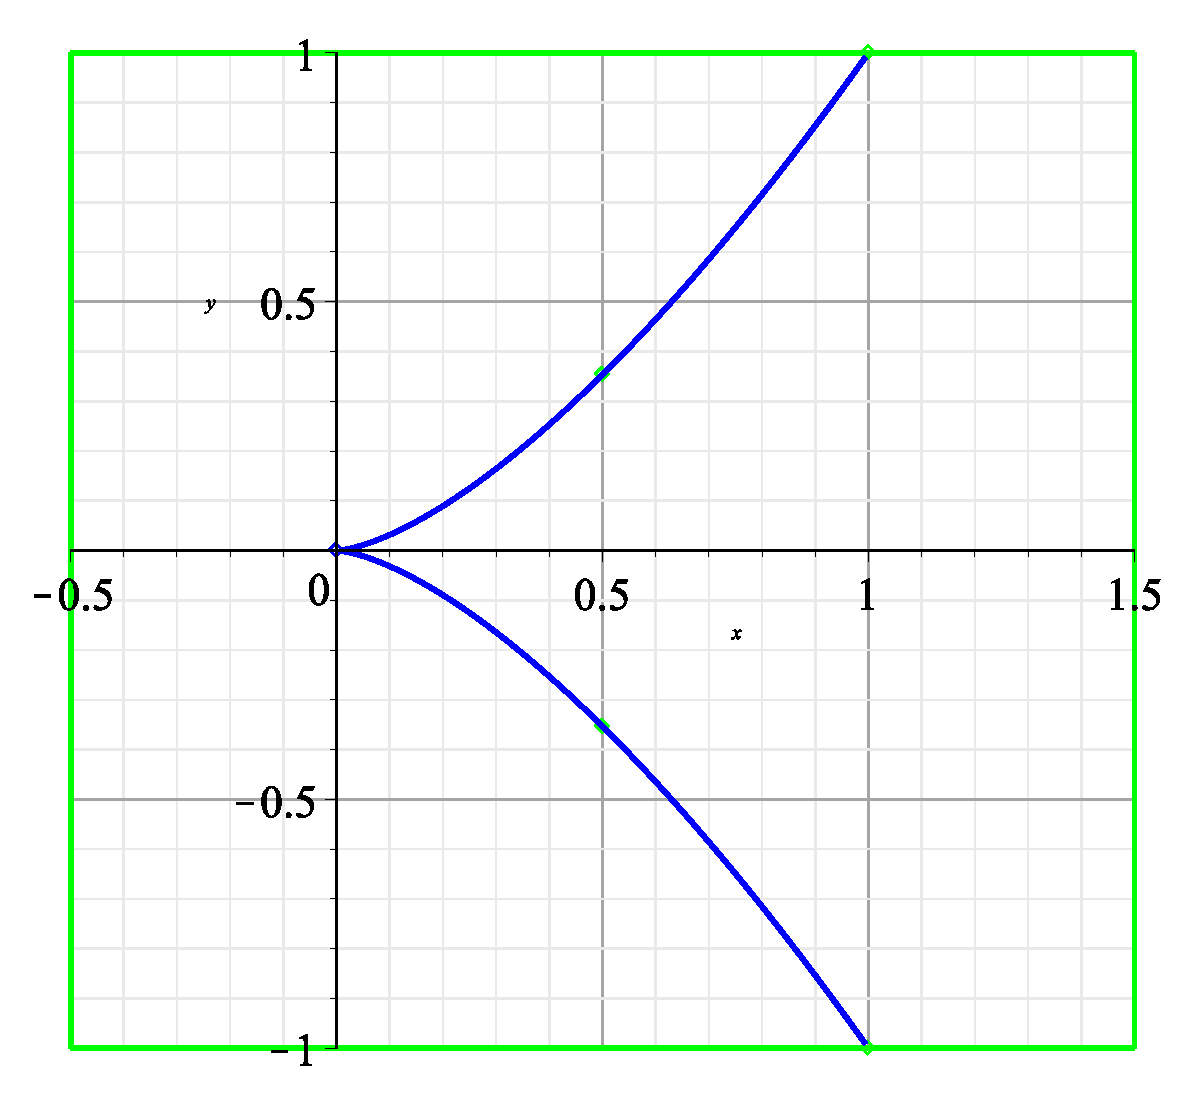
\includegraphics[scale=.3]{img/curve_0_4.eps}
	\caption{Die Kurven $C_1$ (links) und $C_2$ (rechts). $C_1$ ist nicht glatt im Punkt $(1,1)$, $C_2$ nicht im Punkt $(0,0)$.}
	\label{fig:bsp}
\end{figure}

Für die Kryptographie sind elliptische Kurven interessant, weil sich eine Verknüpfung auf ihrer Punktemenge definieren lässt, mit der diese zu einer Gruppe wird. Dabei gerade auch endliche Körper $k$ zuzulassen, macht diese Verknüpfung auf Rechenmaschinen realisierbar. Die Sicherheit der darauf beruhenden elliptic curve cryptography (ECC) beruht darauf, dass das Problem des diskreten Logarithmus auf einer elliptischen Kurve $E$, nämlich die Umkehrung der Funktion $P \mapsto mP$ für $m \in \NN$ fest, nach heutigem Wissensstand rechnerisch im Allgemeinen extrem schwer realisierbar ist.
\newpage
\section{Fundamentalsatz der elementaren Arithmetik}
\label{sec:para1}

\minisec{Terminologie}
	Sei $R$ ein kommutativer Ring mit $1 \neq 0$. $R$ heißt \Index{Integritätsring} bzw. \bet{nullteilerfrei}, wenn gilt: \index{Nullteiler} \marginnote{14.10.}
	\[ a \cdot b = 0 \quad \Rightarrow \quad a = 0 \text{ oder } b = 0.\]

\begin{bsp} \label{bsp_integritaetsringe}
	\begin{itemize}
		\item $\ZZ$
		\item $\ZZ[\sqrt{2}] := \{a + b\sqrt{2} : a,b \in \ZZ \} \subseteq \RR$ \\
			$\ZZ[i] := \{a + bi : a,b \in \ZZ\} \subseteq \CC$ \\
			$\ZZ[\sqrt{-5}] := \dots$
		\item $K[X]$ für $K$ Körper \\
			$\ZZ[X]$
		\item $K$ Körper
		\item $\CC \sprod{z} := \penbrace{\text{konvergente Potenzreihen } \sum\limits_{n=0}^{\infty} a_n z^n}$
		\item Nicht nullteilerfrei ist z.B. $\mathcal{C}[0,1] := \{f \colon [0,1] \rightarrow \RR \text{ stetig} \}$
	\end{itemize}
\end{bsp}

\begin{defn}[Teilbarkeit] \label{def_1.1}
	Seien $a,b \in R$. $a$ heißt ein \Index{Teiler} von $b$, wenn ein $q \in R$ existiert mit $b = qa$, und schreiben:
	\[ a | b \]
	Ist $R$ nullteilerfrei und $a \neq 0$, so ist $q$ eindeutig bestimmt.
\end{defn}

\begin{falko}[Triviale Teilbarkeitsregeln] \label{F1.1}
	\begin{enumerate}[(i)]
		\item $a | 0, 1 | a, a | a$
		\item $a | b, b | c \quad \Rightarrow \quad a | c$
		\item $a | b, a | c \quad \Rightarrow \quad a | b+c, a | b-c$
		\item $a_1 | b_1, a_2 | b_2 \quad \Rightarrow \quad a_1 a_2 | b_1 b_2$
		\item $ac | bc \quad \Rightarrow \quad a | b$, falls $c \neq 0$ und $R$ nullteilerfrei.
	\end{enumerate}	
\end{falko}

\begin{defn}[Einheit, assoziiert] \label{def_1.2}
	\begin{enumerate}[(i)]
		\item $e \in R$ heißt eine \Index{Einheit} in $R$, falls $e | 1$ gilt, d.h. falls ein $f \in R$ existiert mit $ef = 1$. $f$ ist eindeutig bestimmt. Wir setzen $e^{-1} := f$ und schreiben auch $\frac{1}{e}$ für $e^{-1}$. \\
		Wir bezeichnen die \Index{Einheitengruppe} von $R$ mit $R^\times := \{x \in R : x \text{ ist Einheit in } R\}$.
		\item $a \in R$ heißt \Index{assoziiert} zu $b \in R$, falls $a | b$ und $b | a$ gilt. Schreibe: $a \assoz b$.
	\end{enumerate}
\end{defn}

\begin{bsp}
	\begin{enumerate}[1)]
		\item Sei $K$ ein Körper, dann ist $K^\times = K \setminus \setnull$. \qquad $\ZZ^\times = \{1,-1\}$, \qquad $K[X]^\times = K^\times$, \\
		$\mathcal{C}[0,1]^\times = \{f \in \mathcal{C}[0,1] : f(x) \neq 0 \text{ für alle } x \in [0,1]\}$, \qquad  $\ZZ[\sqrt{2}]^\times = \{\pm (1+\sqrt{2})^k : k \in \ZZ \}$ \\
		$\ZZ[X]^\times = \{1, -1\}$ \qquad $\CC \sprod{z}^\times = \penbrace*{ \sum a_n z^n \in \CC \sprod{z} : a_0 \neq 0}$
		\item $e \in R^\times \quad \Leftrightarrow \quad e | a$ für jedes $a \in R$.
	\end{enumerate}
\end{bsp}

\begin{falko} \label{F1.2}
	Sei $R$ ein Integritätsring, $a, b \in R$ und $b \neq 0$. Dann gilt:
	\[ a \assoz b \quad \Leftrightarrow \quad \exists e \in R^\times \text{ mit } b = ea \]
\end{falko}

\minisec{Beweis}
	\begin{description}
		\item[\bewrueck] $a | b, e^{-1}b = a, b | a$
		\item[\bewhin] Da $a | b$ und $b | a$, existieren $e, f \in R$, sodass $b = ea$ und $a = fb$. $\Rightarrow b = efb \Rightarrow ef = 1$, da $b \neq 0$ und $R$ nullteilerfrei. \qed
	\end{description}

\setlength{\fboxsep}{10pt}
\setlength{\fboxrule}{3pt}
\begin{center}
	\fbox{\textbf{Ab jetzt ist, wenn nichts anderes gesagt, $R$ ein Integritätsring!}}
\end{center}

\begin{defn}[unzerlegbar, irreduzibel, zusammengesetzt] \label{def_1.3}
	Sei $a \in R \setminus R^\times$. $a$ heißt \Index{unzerlegbar} oder \Index{irreduzibel} in $R$, wenn gilt:
	\[ a = bc \text{ in } R \quad \Rightarrow \quad b \in R^\times \text{ oder } c \in R^\times. \]
	Andernfalls heißt $a$ \bet{zerlegbar}, \bet{zusammengesetzt} oder \bet{reduzibel}.
\end{defn}

\minisec{Bemerkung}
	$a$ unzerlegbar $\quad \Leftrightarrow \quad $ jeder Teiler von $a$ ist Einheit oder assoziiert zu $a$ \\
	$a$ zerlegbar $\quad \Leftrightarrow \quad a$ hat echten Teiler, d.h. einen Teiler, der weder eine Einheit ist noch assoziiert zu $a$

\setcounter{countdef}{2}
\begin{defn}[Primzahl] \label{def_1.3'}
	Ein $p \in \ZZ$ heißt \Index{Primzahl}, wenn $p \in \NN$ und $p$ unzerlegbar in $\ZZ$. Wir beziechnen mit $\PP$ die Menge der Primzahlen von $\ZZ$. $a$ unzerlegbar in $\ZZ \Leftrightarrow a = p$ oder $a = -p$ mit $p \in \PP$.
\end{defn}

\minisec{Bemerkung}
	$a \in \ZZ$ sei zerlegbar, $a \neq 0$. Dann gibt es eine Primzahl $p$ mit $p | a$ und $p \leq \sqrt{|a|}$.

\begin{defn}[Zerlegung in unzerlegbare Faktoren] \label{def_1.4}
	Wir sagen, $a \in R$ besitzt in $R$ eine \Index{Zerlegung in unzerlegbare Faktoren}, wenn
	\begin{equation}
	\begin{aligned}
		a = ep_1p_2\dots p_r \text{ mit } e \in R^\times \text{ und } p_1,\dots,p_r \text{ unzerlegbar} \label{eq_def_1.4}
	\end{aligned}
	\end{equation}
	\eqref{eq_def_1.4} heißt eine Zerlegung von $a$ in unzerlegbare Faktoren. Auch $r = 0$ ist erlaubt.
\end{defn}

\begin{falko} \label{F1.3}
	In $\ZZ$ besitzt jedes $a \neq 0$ eine Zerlegung in unzerlegbare Faktoren.
\end{falko}	

\setcounter{countfalko}{2}
\begin{falko} \label{F1.3'}
	Jede natürliche Zahl $a > 1$ besitzt eine Zerlegung $a = p_1p_2 \dots p_r$ mit Primzahlen $p_1,\dots,p_r$ und $r \geq 1$.
\end{falko}

\minisec{Bemerkung}
	\begin{enumerate}[1)]
		\item Die Aussage F1.3 gilt auch für die Beispiele zu Beginn, mit Ausnahme von $\mathcal{C}[0,1]$.
		\item Sei $R$ ein Integritätsring, der die \Index{Teilbarkeitsbedingung für Hauptideale} erfüllt, so besitzt jedes $a \neq 0$ aus $R$ eine Zerlegung in unzerlegbare Faktoren.
		\item Primzahlen sind die multiplikativen Bausteine (Atome) von $\NN$.
		\item Im Beispiel $\CC\sprod{z}$ von oben gibt es (bis auf Assoziiertheit) nur das einzige unzerlegbare Element $z$. Dieses ist ein \Index{Primelement} (der Begriff folgt weiter unten).
	\end{enumerate}
	
\begin{satz}[Existenz unendlich vieler Primzahlen] \label{satz_1.1}
	Es gibt unendlich viele Primzahlen.
\end{satz}

\textbf{Bemerkungen} \\
	Es sei $p_1,p_2,\dots$ die aufsteigend sortierte Folge der Primzahlen.
	\begin{enumerate}[1)]
		\item $a_n := p_1p_2\dots p_n +1$ ist Primzahl für $n \leq 5$, aber z.B. nicht für $n = 6$. Unklar ist, ob unendlich viele $a_n$ Primzahlen oder keine Primzahlen sind.
		\item Für $x \in \RR_{>0}$ definieren wir:
		\[ \pi(x) := \# \penbrace{p \in \PP : p \leq x}\]
	\end{enumerate}

\minisec{Primzahlsatz (Gauß, Legendre)}
	\begin{equation}
		\pi(x) \sim \frac{x}{\log x}, \text{ d.h. } \lim\limits_{x \rightarrow \infty} \frac{\pi(x)}{x / \log x} = 1 \label{eq_primzahlsatz1}
	\end{equation}
	\begin{equation}
		\pi(x) \sim \int_{2}^{x} \frac{1}{\log t} dt =: \li(x) \label{eq_primzahlsatz_2}
	\end{equation}
	\begin{equation}
	\pi(x) > \frac{x}{\log x} \text{ für alle } x \geq 17 \label{eq_primzahlsatz_3}
	\end{equation}
	\begin{equation}
	\pi(n) > \frac{n}{\log n} \text{ für alle } n \in \NN, n \geq 11 \label{eq_primzahlsatz_4}
	\end{equation}
	
\begin{defn}[eindeutige Zerlegung] \label{def_1.5}
	Sei $R$ ein kommutativer Ring mit $1 \neq 0$. Wir sagen, $a \in R \setminus \setnull$ hat eine \bet{eindeutige} \Index{Zerlegung in unzerlegbare Faktoren}, wenn $a$ eine Zerlegung
	\[ a = ep_1p_2 \dots p_r \]
	in unzerlegbare Faktoren besitzt und eine solche im folgendem Sinne eindeutig ist: Ist auch
	\[ a = e'p_1'p_2'\dots p'_{r'} \]
	eine solche Zerlegung, so gilt $r = r'$ und nach Umnummerierung $p_i' \assoz p_i$ für alle $1 \leq i \leq r$.
\end{defn}

\begin{falko}\label{F1.4}
	In dem Integritätsring $R$ besitze jedes Element $a \neq 0$ eine Zerlegung in unzerlegbare Faktoren. Dann sind äquivalent: \begin{enumerate}[(i)]
		\item Jedes $a \neq 0$ aus $R$ hat eindeutige Zerlegung in unzerlegbare Faktoren.
		\item Ist $p$ unzerlegbar, so gilt: $p | ab \Rightarrow p | a$ oder $p | b$.
	\end{enumerate}
\end{falko}

\begin{defn}[Primelement] \label{def_1.6}
	Sei $R$ ein kommutativer Ring mit $1 \neq 0$. Ein $p \in R\setminus R^\times$ heißt \Index{Primelement} von $R$, wenn für alle $a, b \in R$ gilt:
	\begin{equation}
		p | ab \quad \Leftrightarrow \quad p | a \text{ oder } p | b \label{eq_def_1.6}
	\end{equation}
\end{defn}

\minisec{Bemerkung}
	\begin{enumerate}[1)]
		\item $0$ ist Primelement in $R \Leftrightarrow R$ ist Integritätsring
		\item In einem Integritätsring $R$ gilt: Jedes Primelement $p \neq 0$ ist unzerlegbar.
	\end{enumerate}

\begin{lemma}
	Seien $a, b \in \NN$. Sei $m = \kgV(a,b) \in \NN$. Dann gilt:
	\[ a|c \text{ und } b|c \quad \Rightarrow \quad m | c \]
	$m$ ist also auch minimal bzgl. der Teilbarkeitsrelation $|$.
\end{lemma}

\begin{falko}[Satz von Euklid] \label{F1.5}
	Jede Primzahl $p$ ist ein Primelement von $\ZZ$, d.h. es gilt stets \eqref{eq_def_1.6}. (Das gleiche gilt für $-p$, also für jedes unzerlegbare Element von $\ZZ$.) \index{Satz von Euklid}
\end{falko}

\minisec{Fundamentalsatz der elementaren Arithmetik}
	In $\ZZ$ hat jedes $a \neq 0$ eine eindeutige Zerlegung in unzerlegbare Faktoren. \index{Fundamentalsatz der elementaren Arithmetik}

\minisec{Bemerkung}
	Eindeutige Zerlegung in unzerlegbare Faktoren hat man zum Beispiel auch für die Ringe $\ZZ[\sqrt{2}], \ZZ[i], K[X]$ und $K$ für $K$ Körper, $\ZZ[X]$ und $\CC\sprod{z}$, nicht aber für $\ZZ[\sqrt{-5}]$:
	\[ 3 \cdot 3 = 9 = (2+ \sqrt{-5})(2 - \sqrt{-5}) \]
	Dies sind zwei wesentlich verschiedene Zerlegungen in unzerlegbare Faktoren.

\begin{defn}[Exponent] \label{def_1.7}
	Sei $p$ eine Primzahl und $a \in \ZZ \setminus \setnull$. Dann heißt
	\[ w_p(a) :=\max\{k \in \NN_0 : p^k |a \} \]
	der \Index{Exponent} von $p$ in $a$. Wir setzen $w_p(0) := \infty$.
\end{defn}

\begin{falko}[Eigenschaften der Exponentfunktion] \label{F1.6}
	Die Funktion $w_p \colon \ZZ \rightarrow \NN_0 \cup \{\infty\}$ hat folgende Eigenschaften:
	\begin{enumerate}[(i)]
		\item $w_p(a+b) \geq \min(w_p(a),w_p(b))$ und Gleichheit, falls $w_p(a) \neq w_p(b)$.
		\item $w_p(ab) = w_p(a) + w_p(b)$
	\end{enumerate}
\end{falko}

\begin{satz}[Fundamentalsatz der elementaren Arithmetik] \label{satz_1.2}
	Für jedes $a \in \ZZ \setminus \setnull$ gilt $w_p(a) > 0$ nur für endlich viele $p$. Es ist
	\begin{equation}
		a = \sgn(a) \cdot \prod\limits_p^{} p^{w_p(a)} \label{eq_satz_1.2}
	\end{equation}
\end{satz}

\minisec{Bemerkung}
	\begin{enumerate}[1)]
		\item $w_p$ lässt sich eindeutig zu einer Abbildung $w_p \colon \QQ \rightarrow \ZZ \cup \{\infty\}$ fortsetzen, sodass (ii) für alle $a,b \in \QQ$ gilt. Es gilt dann auch (i). Für $a \in \QQ \setminus \setnull$ ist $w_p(a) \neq 0$ nur für endlich viele $p$, und die Formel \eqref{eq_satz_1.2} gilt entsprechend.  Ferner gilt: $a \in \ZZ \Leftrightarrow w_p(a) \geq 0$ für alle $p$.
		\item Sei
		\[ \NN_0^{(\PP)} := \{ (e_p)_{p \in \PP} : e_p \in \NN_0, e_p = 0 \text{ für fast alle } p \}. \]
		Nach Satz \ref{satz_1.2} sind $(\NN,\cdot)$ und $(\NN_0^{(\PP)},+)$ zwei zueinander isomorphe Halbgruppen. Nach Bemerkung 1) sind $\QQ^\times$ und $\{1,-1\} \times \ZZ^{(\PP)}$ sogar zwei zueinander isomorphe Gruppen.
	\end{enumerate}
	
\begin{defn}[faktorieller Ring, Vertretersystem für Primelemente] \label{def_1.8}
	Ein Integritätsring $R$ heißt \Index{faktoriell}, wenn jedes $a \in R \setminus \setnull$ eine eindeutige Zerlegung in unzerlegbare Faktoren hat. Man spricht dann auch von eindeutiger Primfaktorzerlegung in $R$. \\
	$P$ heißt \bet{Vertretersystem für die Primelemente $\neq 0$} von $R$, wenn:
	\begin{enumerate}[(1)]
		\item Zu jedem Primelement $q \neq 0$ von $R$ gibt es ein $p \in P$ mit $q \assoz p$. 
		\item Für $p, p' \in P$ mit $p \assoz p'$ gilt $p = p'$, d.h. $p$ in (1) ist eindeutig bestimmt durch $q$.
	\end{enumerate}
	Für $R = \ZZ$ nehme man stets $P = \PP$. Für $K$ Körper und $R = K[X]$ nimmt man $P = \{p \in K[X] : p \text{ irreduzibel und normiert}\}$. \index{Primelement} \index{Vertretersystem}
\end{defn}

\begin{falko} \label{F1.7}
	Sei $R$ faktoriell und $P$ ein Vertretersystem für Primelemente. Es gibt zu jedem $p \in P$ eine Funktion $w_p \colon R \rightarrow \NN_0 \cup \{\infty\}$ mit den Eigenschaften (i) und (ii) aus F\ref{F1.6}, sodass gilt: \begin{enumerate}[a)]
		\item Für jedes $a \in R \setminus \setnull$ ist $w_p(a) > 0$ nur für endlich viele $p \in P$.
		\item Für jedes $a \in R \setminus \setnull$ gilt
		\begin{equation}
			a = e \prod\limits_{p \in P}^{} p^{w_p(a)} \label{eq_F1.7}
		\end{equation}
		mit eindeutigem $e \in \RR^\times$.
	\end{enumerate}
\end{falko}

\begin{defn}[ggT und kgV] \label{def_1.9}
	Sei $R$ ein kommutativer Ring mit $1 \neq 0$. Gegeben $a_1, \dots, a_n \in R$.
	\begin{enumerate}[a)]
		\item Ein $d \in R$ heißt ein \Index{größter gemeinsamer Teiler} (ggT) von $a_1,\dots,a_n$, falls:
		\begin{center}
			1. \quad $d | a_i$ für alle $i$ \hspace{3cm} 2. \quad $t | a_i$ für alle $i \Rightarrow t | d$
		\end{center}
		\item Ein $m \in R$ heißt ein \Index{kleinstes gemeinsames Vielfaches} (kgV) von $a_1,\dots,a_n$, falls:
		\begin{center}
			1. \quad $a_i | m$ für alle $i$ \hspace{3cm} 2. \quad $a_i | c$ für alle $i \Rightarrow m | c$
		\end{center}
	\end{enumerate}
\end{defn}

\minisec{Bemerkung}
	\begin{enumerate}[1)]
		\item $d, d'$ ggT von $a_1, \dots, a_n \Rightarrow d \assoz d'$ und $m, m'$ kgV von $a_1, \dots, a_n \Rightarrow m \assoz m'$
		\item Im Allgemeinen ist die Existenz eines ggT und kgV nicht gesichert. In faktoriellen Ringen existieren sie aber immer, siehe dazu folgende Feststellung.
	\end{enumerate}
\newpage
\section{Elliptische Kurven}
\label{sec:para2}
\nextlecture
\subsection{Grundlagen aus der Algebra}
\subsubsection{Polynome}
	Sei $k$ ein beliebiger Körper. \marginnote{[7]}
	
\begin{defn}[Polynom]
	Ein \Index{Polynom} über $k$ in den $n$ Variablen $x_1,\dots,x_n$ ist ein Ausdruck der Form
	\[ f(x_1,\dots,x_n) = \sum\limits_{\nu_1,\dots,\nu_n \geq 0} \alpha_{\nu_1, \dots, \nu_n} x_1^{\nu_1} \cdots x_n^{\nu_n} \]
	mit Koeffizienten $\alpha_{\nu_1,\dots,\nu_n} \in k$, von denen nur endlich viele $\neq 0$ sind. Hat man es mit mehreren Variablen ($n \geq 2$) zu tun, kann man auch kurz
	\[ f(\underline{x}) = \sum_{\uline{\nu} \in \NN_0^n} \alpha_{\uline{\nu}} x_1^{\nu_1} \cdots x_n^{\nu_n} \]
	schreiben, wenn man die Tupelschreibweise $\uline{\nu} \in \NN_0^n$ bzw. $\uline{x} = (x_1, \dots x_n)$ einführt, wobei man für das Monom $x_1^{\nu_1} \cdots x_n^{\nu_n}$ auch kurz $\uline{x}^{\uline{\nu}}$ schreiben kann, wenn klar ist, dass $n \geq 2$ viele Variablen vorliegen. \\
	Die Menge aller Polynome über $k$ in $n$ Variablen wird kurz mit $k[x_1,\dots,x_n]$ oder noch kürzer mit $k[\uline{x}]$ bezeichnet. Wir schreiben dann auch kurz $f \in k[\uline{x}]$, wenn $f(\uline{x})$ ein Polynom ist.
\end{defn}

\begin{bem}
	Durch eine Addition und Multiplikation definiert durch
	\begin{equation}
	\begin{aligned}
		\sum_{\uline{\nu}} \alpha_{\uline{\nu}} \uline{x}^{\uline{\nu}} + \sum_{\uline{\nu}} \beta_{\uline{\nu}} \uline{x}^{\uline{\nu}} &:= \sum_{\uline{\nu}} (\alpha_{\uline{\nu}} + \beta_{\uline{\nu}}) \uline{x}^{\uline{\nu}} \\
		\enbrace*{\sum_{\uline{\nu}} \alpha_{\uline{\nu}} \uline{x}^{\uline{\nu}}} \cdot \enbrace*{\sum_{\uline{\mu}} \beta_{\uline{\mu}} \uline{x}^{\uline{\mu}}} &:= \sum_{\uline{\nu},\uline{\mu}} \alpha_{\uline{\nu}} \beta_{\uline{\mu}} \uline{x}^{\uline{\nu} + \uline{\mu}}
	\end{aligned}
	\end{equation}
	wird $k[\uline{x}]$ zu einem kommutativen Ring mit Eins; das Nullpolynom $0 := \sum_{\uline{\nu}} 0 \uline{x}^{\uline{\nu}}$ ist dabei das Nullelement, das Polynom $1 := 1 \cdot \uline{x}^{\uline{0}} + \sum_{\uline{\nu} \neq 0} 0 \uline{x}^{\uline{\nu}}$ ist das Einselement. \marginnote{"Einspolynom"} \\
	Der Ring $(k[\uline{x}],+,\cdot)$ heißt \Index{Polynomring} über $k$.
\end{bem}

\begin{defn}[Formale Ableitung]
	Für $f(\uline{x}) = \sum_{\uline{\nu}} \alpha_{\uline{\nu}} \uline{x}^{\uline{\nu}} \in k[\uline{x}]$ und $1 \leq j \leq n$ heißt
	\[ \frac{\der f}{\der x_j}(\uline{x}) := \sum_{\uline{\nu}, \nu_j > 0} \alpha_{\uline{\nu}} v_j x_1^{\nu_1} \cdots x_j^{\nu_j-1} \cdots x_n^{\nu_n} \in k[\uline{x}] \]
	die \Index{formale Ableitung} von $f$ nach $x_j$.
\end{defn}

\begin{satz}[Produktregel, Kettenregel]
\label{satz_7.4}
	Für alle $f,g \in k[\uline{x}]$ und $\gamma \in k$ gelten die Ableitungsregeln
	\[ \frac{\der(\gamma f)}{\der x_j} = \gamma \frac{\der f}{\der x_j} \hspace{2cm} \frac{\der(f+g)}{\der x_j} = \frac{\der f}{\der x_j} + \frac{\der g}{\der x_j} \hspace{2cm} \frac{\der(fg)}{\der x_j} = f \frac{\der g}{\der x_j} + g \frac{\der f}{\der x_j} \]
	und für $f \in k[x_1, \dots,x_m], g_1,\dots, g_m \in k[x_1,\dots, x_n]$
	\[ \frac{\der f(g_1,\dots, g_m)}{\der x_j}(\uline{x}) = \frac{\der f}{\der x_1} (g_1,\dots,g_m) \frac{dg_1}{dx_j}(\uline{x}) + \dots + \frac{\der f}{\der x_m} (g_1,\dots,g_m) \frac{\der g_m}{\der x_j}(\uline{x}). \]
\end{satz}

Polynome in einer Variablen $f \in k[x]$ der Form $f(x) = \sum_{\nu = 0}^{k} \alpha_\nu x^\nu$ sind aus den Grundvorlesungen bekannt.
\begin{defn}[Grad]
	Ist $f \neq 0$, so heißt $\deg(f) := \min\{j \in \NN_0 : a_j \neq 0\}$ der Grad von $f$. Für $f \in k[\uline{x}]$ in $n$ Variablen ist $\deg(f) := \min\{\nu_1 + \dots + \nu_n : a_{\uline{\nu}} \neq 0\}$ der \Index{Grad} von $f$. Neu ist bei uns, dass wir uns hier vor allem mit $n = 2$ oder $n = 3$ Variablen beschäftigen werden, wo wir dann auch $f(x,y)$ oder $f(x,y,z)$ schreiben möchten, zum Beispiel $f(x,y) = \alpha_{(2,0)} x^2 + \alpha_{(1,1)} xy + \alpha_{(0,1)}y$. Wir werden dann für die Koeffizienten einfachere Notationen wählen.
\end{defn}

\begin{bem}
	Bleiben wir zunächst beim Polynomring $k[x]$ in einer Variablen $x$. Sei $f \in k[x]$. Wie im Ring $\ZZ$ können wir Teilbarkeit in $k[x]$ studieren und Divisionen mit Rest durchführen (Polynomdivision), daher kann man wie in $\ZZ$ zum Beispiel den ggT von Polynomen mit dem euklidischen Algorithmus ausrechnen. Dies ist aus den Grundvorlesungen bekannt, wir erinnern hier nur an folgendes:
\end{bem}

\begin{defn}[Nullstelle]
	Gegeben sei die Einsetzabbildung
	\begin{equation}
	\begin{aligned}
		k &\longrightarrow k \\
		c &\longmapsto f(c) := \sum_{\nu = 0}^{k} \alpha_\nu c^\nu
	\end{aligned}
	\end{equation}
	Ein Element $c \in k$ heißt \Index{Nullstelle} von $f$, falls $f(c) = 0$ in $k$ ist.
\end{defn}

\begin{bem}
	$c \in k$ ist genau dann Nullstelle, wenn $(x-c)$ ein Teiler von $f$ im Polynomring $k[x]$ ist, d.h. falls ein $g \in k[x]$ existiert mit $(x-c) \cdot g = f$.
\end{bem}

\begin{defn}[Ordnung einer Nullstelle]
	Ist $c$ eine Nullstelle von $f \neq 0$, so gibt es ein maximales $k \geq 1$, sodass $(x-c)^k$ ein Teiler von $f$ ist. Die Zahl $k$ heißt \bet{Ordnung der Nullstelle} $c$. Ist $f(c) \neq 0$, definiert man diese "Nullstellen"ordnung als $0$. \index{Ordnung!Nullstelle}
\end{defn}

\begin{defn}[irreduzibel, prim]
	Ein Polynom $f \in k[x]$ vom Grad $\geq 1$ heißt \Index{irreduzibel} (oder \bet{prim}), falls gilt: Ist $f = u \cdot v$ mit $u,v \in k[x]$, dann ist $\deg(u) = 0$ oder $\deg(v) = 0$, das heißt $f$ kann nicht als Produkt zweier Polynome vom Grad $\geq 1$ geschrieben werden. (vgl. den Begriff "Primzahl" bei $\ZZ$; der Satz von der eindeutigen Zerlegung in irreduzible Polynome heißt der \Index{Satz von Gauß}.)
\end{defn}

Wenn wir $\ZZ$ als Vorbild für den Polynomring $k[x]$ nehmen, möchten wir auch das "Modulorechnen" auf $k[x]$ übertragen, um neue Strukturen zu erhalten. Unsere Moduln sind dann Polynome:
\begin{defn}[Kongruenz, Restklassenring (Polynome)]
	Sei $f \in k[x]$. Dann heißen $a \in k[x]$ und $b \in k[x]$ \bet{kongruent modulo $f$},\index{Kongruenz!Polynome} wenn $f \mid (b-a)$, das heißt falls ein $g \in k[x]$ existiert mit $b = a + fg$.\marginnote{"$\kon$" nur für $\ZZ$} Die Restklassen modulo $f$ sind Teilmengen von $k[x]$ der Gestalt $a + f \cdot k[x] := \{a + fg : g \in k[x]\}$ mit $a \in k[x]$. Das Polynom $a \in k[x]$ heißt ein \Index{Repräsentant} der Restklasse. Ist der Modul $f \in k[x]$ klar, möchten wir dafür auch kurz wieder $\uline{\uline{a}}$ schreiben.\marginnote{doppelt unterstreichen!} \\
	Die Menge der Restklassen modulo $f$ bezeichnen wir mit
	\[ k[x] / (f) := \{a + f\cdot k[x] : a \in k[x]\} = \{\uline{\uline{a}} : a \in k[x]\} \]
	und nennen diese den \bet{Restklassenring modulo $f$}, weil diese bezüglich der Definition $\uline{\uline{a}} + \uline{\uline{b}} := \uline{\uline{a+b}}$ (analog für Multiplikation) für Polynome $a,b \in k[x]$ wieder zu einem kommutativen Ring mit $\uline{\uline{1}}$ als Eins wird. \index{Restklasse!Polynom}
\end{defn}

Doch die einfache Frage, wie viele Elemente der Restklassenring hat, hängt unter anderem vom Körper $k$ ab. Im Fall $k = \FF_p$ beantworten wir diese. Klar ist wegen der Teilbarkeit mit Rest im Ring $k[x]$ (d.h. sind $b,f \in k[x]$ und $f \neq 0$, so existieren eindeutige $g,r \in k[x]$ mit $r = 0$ oder $\deg(r) < \deg(f)$,\marginnote{Polynomdivision} sodass $b = f\cdot g + r$ gilt):
\begin{bem}
\label{bem_7.12}
	Für jede Restklasse $\uline{\uline{a}} = a + f \cdot k[x] \in k[x]/(f)$ gibt es genau einen Vertreter $b \in \uline{\uline{a}} = a + f\cdot k[x]$, das heißt $\uline{\uline{b}} = \uline{\uline{a}}$ bzw. $b + f \cdot k[x] = a + f \cdot k[x]$, mit $b = 0$ oder $\deg(b) < \deg(f)$.
\end{bem}

\subsubsection{Endliche Körper}
\label{subsub:2.1.2}
	Sei nun $k = \FF_p$ mit $p$ prim.

\begin{satz}
	Sei $f \in \FF_p[x]$ irreduzibel mit $r := \deg(f)$. Dann ist $\FF_p[x]/(f)$ ein Körper mit $p^r$ Elementen.
\end{satz}

\minisec{Beweis}
	Dass $\FF_p[x]/(f)$ ein Körper ist, ist klar (Inverse findet man mit dem euklidischen Algorithmus). $\FF_p[x]$ hat $p^r$ Elemente, denn jede Restklasse hat genau einen Vertreter
	\[ b = \underbrace{\alpha_0 + \dots + a_{r-1} x^{r-1}}_{p \text{ Möglichkeiten für jedes } \alpha_j} \qed\]
	
\begin{bem}
	Für jedes $r \in \NN$ gibt es (mindestens) ein irreduzibles Polynom $f \in \FF_p[x]$ mit $\deg(f) = r$.
\end{bem}

\begin{bem}
	Es gibt im Wesentlichen (das heißt bis auf Isomorphie) genau einen endlichen Körper mit $p^r$ Elementen, das heißt welches irreduzible $f$ mit $\deg(f) = r$ wir als Modul nehmen, ist für seine Konstruktion (bis auf Isomorphie!) egal. Wir bezeichnen diesen Körper mit $\FF_{p^r}$.
\end{bem}

\begin{bem}
	Jeder Körper mit endlich vielen Elementen ist einer dieser Körper $\FF_{p^r}$ mit $p$ prim und $r \geq 1$. (ohne Beweis, vgl. Vorlesung "Einführung in die Algebra")
\end{bem}

\begin{bem}
	Wegen Bemerkung \ref{bem_7.12} ist nach Wahl eines irreduziblen Polynom $f \in \FF_p[x], \deg(f) = r$ also
	\[\FF_{p^r} = \{ (\alpha_{r-1} x^{r-1} + \dots + \alpha_1 x + \alpha_0) + f \cdot \FF_p[x] : \alpha_i \in \FF_p\},\]
	die Restklassenvertreter $\alpha_{r-1} x^{r-1} + \dots + \alpha_1 x + \alpha_0$ lassen sich auch durch Koeffizienten-$r$-Tupel $(\alpha_{r-1}, \alpha_{r-2}, \dots, \alpha_1, \alpha_0) \in \FF_{p^r}$ darstellen. Will man mit ihnen stellvertretend für die Polynomrestklassen in $\FF_{p^r}$ rechnen, muss man also erst mit den zugehörigen Polynomen über $\FF_p$ rechnen und modulo $f$ reduzieren.
\end{bem}

\begin{bsp}
	Sei $p = 2, r=3$, wir möchten $\FF_8$ konstruieren.\marginnote{Unterstreichungen weggelassen!} Das Polynom $f(x) = x^3 + x + 1$ ist irreduzibel über $\FF_2 = \{0,1\}$, also ist 
	\[ \FF_8 = \FF_2[x]/(f) = \{ (0,0,0), (0,0,1), (0,1,0), (0,1,1), (1,0,0), (1,0,1), (1,1,0), (1,1,1)\}, \]
	und man rechnet zum Beispiel $(0,1,0) \cdot (1,1,1) = (1,0,1)$, weil
	\[ (0x^2 + 1x + 0) \cdot (x^2 + x + 1) = x^3 + x^2 + x = 1 \cdot (x^3 + x + 1) + (x^2 + 1) \]
	in $\FF_2[x]$ gilt (Division mit Rest durch $f$). \begin{itemize}
	\item Bei Wahl des irreduziblen Polynoms $f(x) = x^3 + x^2 + 1$ ergeben sich zwar andere Rechenregeln für die Vektorenmultiplikation, man erhält aber die selbe "Struktur" bei $+,\cdot$ mit entsprechenden Elementen. Stellen Sie als Übung mal die Multiplikations- und Additionstabellen auf, der Einfachheit halber auch erst mal von $\FF_4$.
	\item Streng genommen müsste man zum Beispiel $\uline{\uline{(\uline{1}, \uline{0}, \uline{1})}} = \uline{\uline{x^2 + \uline{1}}}$ für die Elemente von $\FF_8$ schreiben, um die Reduktion modulo $f$ zu verdeutlichen.
	\end{itemize}
\end{bsp}

\begin{bsp}
	Rechnen in $\FF_{5^3} = \FF_{125}$: Haben wir diesen Körper mit dem irreduziblen Polynom $f = x^3 + x + 1 \in \FF_5[x]$ vom Grad $3$ konstruiert,\marginnote{irreduzibel, da keine Nullstelle und Grad 3!} so rechnen wir in $\FF_{5^3}$ zum Beispiel
	\begin{equation}
	\begin{aligned}
		(1,2,4) \cdot (-1,3,0) &= (x^2 + 2x - 1)(-x^2 + 3x) = -x^4 + 3x^3 - 2x^3 + 6x + x^2 -3x \\
		&= -x^4 + x^3 + x^2 + 3x = (x^3+x+1) \cdot (-x+1) + 2x^2+3x+1 = (2,3,1) \modu f
	\end{aligned}
	\end{equation}
\end{bsp}

\begin{bem}
	Es ist $\Char(\FF_{p^r}) = p$, denn es gilt $\uline{1} + \uline{1} + \dots + \uline{1} = \uline{p \cdot 1} = \uline{0}$, und $p$ ist minimal mit dieser Eigenschaft, da prim.
\end{bem}

\begin{defn}[algebraisch abgeschlossen]
	Ein Körper $k$ ist \Index{algebraisch abgeschlossen}, wenn sich jedes Polynom $f \in k[x], \deg(f) > 0$, als Produkt von linearen Polynomen schreiben lässt, das heißt wenn $f(x) = d(x-c_1) \cdots (x-c_m)$ mit $d,c_i \in k$ gilt.
\end{defn}

\begin{bem}
\label{bem_7.22}
	Man kann jeden Körper $k$ in einen algebraisch abgeschlossenen Körper einbetten. Ein bezüglich "$\subseteq$" minimaler heißt algebraischer Abschluss von $k$, dieser ist eindeutig und wird mit $\overline{k}$ bezeichnet. So ist etwa $\overline{\RR} = \CC$. Der algebraische Abschluss $\overline{\FF_p}$ enthält jeden der Körper $\FF_{p^r}, r \geq 1$, und umgekehrt ist jedes Element von $\overline{\FF_p}$ schon in einem dieser Körper $\FF_{p^r}, r \geq 1$, enthalten. (ohne Beweis)
\end{bem}

\nextlecture
\newpage
\subsection{Der affine Raum, affine Kurven und der projektive Raum}
	Wir stellen den zweidimensionalen affinen und projektiven Raum vor,\marginnote{[8]} das heißt die wohlbekannte affine Ebene $k^2 = k \times k$ und ihre Ergänzung zur projektiven Ebene $\PP^2(k)$ durch "unendlich ferne Punkte". Kurven im Affinen, wie zum Beispiel elliptische Kurven werden dann in der projektiven Ebene intergriert, weil es rechentechnisch einfacher und mathematisch natürlicher ist.
	
\subsubsection{Der affine und projektive Raum}
	Sei $k$ ein beliebiger Körper. Wir stellen uns meistens $\RR$ vor, weil wir über geometrische Objekte nachdenken möchten; $k$ ist in den Anwendungen aber meist ein endlicher Körper.

\begin{defn}[zweidimensionaler affiner Raum]
	Den zweidimensionalen $k$-Vektorraum $k^2 = k \times k$ schreiben wir auch als $\aff^2(k) := \{(x_1,x_2) : x_1,x_2 \in k\}$ und nennen ihn den \bet{zweidimensionalen affinen Raum} über $k$ bzw. \bet{affine Ebene} über $k$. \index{affiner Raum}
\end{defn}

\begin{defn}[Gerade]
	Eine \Index{Gerade} in $\aff^2(k)$ ist eine Teilmenge der Form
	\[ g(a,b,c) := \{(x,y) \in \aff^2(k) : ax + by + c = 0\} \subseteq \aff^2(k) \]
	für ein Tripel $(a,b,c) \in k^3$ mit $a,b \neq 0$.
\end{defn}

\begin{bem}
	Zwei verschiedene Geraden in $\aff^2(k)$ schneiden sich in genau einem Punkt, es sei denn, sie sind parallel, das heißt dann haben sie keinen gemeinsamen Punkt in $\aff^2(k)$. Soweit nichts Neues.
\end{bem}

\begin{bem}
	Die Ausnahme, dass in der "Ebene" $k \times k$ Geraden parallel sein können, möchten wir uns beim Rechnen gerne ersparen. Wir ergänzen die Ebene um "unendlich ferne Punkte" und erklären, dass sich zwei parallele Geraden in genau so einem Punkt schneiden. Durch diese Ergänzung wird die affine Ebene zur \bet{projektiven Ebene}. Wie kann das sinnvoll so umgesetzt werden, dass alle Punkte Koordinaten bekommen, mit denen man wie üblich rechnen kann, sodass bei der Schnittpunktberechnung auch die unendlich fernen Punkte erhalten werden können?
	\begin{figure}[h]
		\centering
		\begin{tikzpicture}
			\foreach \x in {0,1,2,3} {
				\draw (-.2,\x) -- (3.2,\x);
				\draw (\x,-.2) -- (\x,3.2);
			}
			\draw[color=blue,very thick] (.5,.2) -- (1.5,.2) -- (1.5,1.2) -- (1,1.9) -- (.5,1.2) -- (.5,.2);
			
			\draw [ultra thick,->] (4,1.5) -- (6,1.5);
		\end{tikzpicture} \hspace{.3cm}
		\begin{tikzpicture}[scale=1.2]
			\draw (-.2,0) -- (3.2,0);
			\draw (.1,.8) -- (2.9,.8);
			\draw (.4,1.4) -- (2.6,1.4);
			\draw (.7,1.9) -- (2.3,1.9);
			
			\draw (-.1,-.1) -- (.9,2.1);
			\draw (.95,-.1) -- (1.3,2.1);
			\draw (2.05,-.1) -- (1.7,2.1);
			\draw (3.1,-.1) -- (2.1,2.1);
			
			\draw [color=blue, very thick] (.55,.15) -- (.78,.9) -- (1.177,1.3) -- (1.5,.9) -- (1.48,.15) -- (.55,.15);
			\draw [thick,->] (1.1,2.0) -- (1.3,2.5);
			\draw [thick,->] (1.9,2.0) -- (1.7,2.5);
			\draw (1.5,2.55) node[above]{$\infty$};
		\end{tikzpicture}
		\caption{Ergänzung des zweidimensionalen affinen Raums zur projektiven Ebene.}
	\end{figure}
\end{bem}

Zwei Parallelen $g(a,1,c)$ und $g(a,1,d)$ sollen sich dann schneiden, auch rechnerisch. Wir lösen das so, dass in unserer neuen "Ebene" eine dritte "Koordinate" $z$ hinzukommt, welche bei diesen Parallelen also $=0$ sein müsste, wie folgt:

\begin{defn}[projektive Ebene]
	Die \Index{projektive Ebene} über $k$ ist die Menge
	\[ \PP^2(k) = \{ [y_1 : y_2 : y_3] : y_i \in k \text{ nicht alle } 0\}\]
	mit der Vereinbarung, dass $[y_1 : y_2 : y_3] = [z_1 : z_2 : z_3]$ genau dann gilt, wenn es ein $\lambda \in k \setminus \setnull$ gibt mit $y_1 = \lambda z_1, y_2 = \lambda z_2$ und $y_3 = \lambda z_3$.
\end{defn}

\begin{defn}[projektive Ebene (formal)]
	$\PP^2(k)$ ist die Menge der Äquivalenzklassen in $k^3$ bezüglich der Äquivalenzrelation
	\[ (y_1,y_2,y_3) \sim (z_1,z_2,z_3) \quad :\Leftrightarrow \quad \exists \lambda \in k \setminus \setnull : y_i = \lambda z_i, i = 1, 2, 3 \]
	das heißt $\PP^2(k) := (k^3 \setminus \{(0,0,0)\} / \sim$. \\
	Wir schreiben $[y_1 : y_2 : y_3]$ für die Äquivalenzklasse, die von $(y_1,y_2,y_3)$ repräsentiert wird und nennen sie einen \bet{projektiven Punkt}. $y_1,y_2,y_3$ nennen wir \bet{projektive Koordinaten} von $[y_1: y_2 : y_3]$.
\end{defn}

\begin{bem}
	Ist $y_3 \neq 0$, gilt $[y_1 : y_2 : y_3] = \benbrace*{\frac{y_1}{y_3} : \frac{y_2}{y_3} : 1}$, das heißt die dritte (oder jede andere Koordinate $\neq 0$) kann dann auf $1$ gebracht ("normiert") werden.
\end{bem}

Einem projektiven Punkt $[x:y:z]$ entspricht in unserem Modell in $k^3$ die Ursprungsgerade $\{(\lambda x, \lambda y, \lambda z) : \lambda \in k\}$. Diese Punkte sind entweder $[x:y:1]$ oder $[x:y:0]$ mit $x,y \in k$ (nicht $[0:0:0]$!). \\
Zum Beispiel durch die Abbildung
\begin{equation}
\begin{aligned}
	\iota\colon \aff^2(k) &\longrightarrow \PP^2(k) \\
	(x,y) &\longmapsto [x:y:1]
\end{aligned}
\end{equation}
kann die affine Ebene in die projektive eingebettet werden (d.h. $\iota$ ist injektiv).
\begin{figure}[h]
	\centering
	\begin{tikzpicture}
		\draw [thick] (.2,-.2) -- (-1,1);
		\draw [thick] (0,-.3) -- (0,1);
		\draw [thick] (-.2,-.2) -- (1,1);
		
		\draw [fill=white] (-1.5,.8) -- (1.5,.8) -- (1.7,1.2) -- (-1.3,1.2) -- (-1.5,.8);
		
		\draw (-1,1) node[fill,circle,inner sep=1pt]{};
		\draw (0,1) node[fill,circle,inner sep=1pt]{};
		\draw (1,1) node[fill,circle,inner sep=1pt]{};
		\draw (0,0) node[fill,circle,inner sep=1pt]{};
		
		\draw [thick, ->] (-1,1) -- (-2,2);
		\draw [thick, ->] (0,1) -- (0,2.2);
		\draw [thick, ->] (1,1) -- (2,2);
		
		\draw (1.7,1) node[align=left,label={right:$\iota(\aff^2(k))$}] {};
		\draw (.1,0) node[right,align=left] {$\leftarrow$ Ursprung};
	\end{tikzpicture}
\end{figure}

\begin{bem}
	Aber $\PP^2(k)$ enthält zusätzlich noch die projektiven Punkte $[x:y:0]$ mit $x,y \in k$ (nicht $x=y=0$). Offenbar ist $\{[x:y:0] : x,y \in k, \text{ nicht } x = y = 0\}$ eine Gerade in $\PP^2(k)$, die wir \Index{unendlich ferne Gerade} $g_\infty$ nennen möchten, denn mit $j \colon k \rightarrow g_\infty, x \mapsto [x:1:0]$ lässt sich $k$ darin einbetten (das heißt $j$ ist injektiv), wobei auffällt, dass $g_\infty \setminus \im(j)$ aus genau den weiteren Punkt $\oh := [1:0:0]$ besteht, das heißt $g_\infty \setminus \im(j) = \{\oh\}$.
\end{bem}

\begin{bem}
	Somit: $\PP^2(k) = \iota(\aff^2(k)) \sqcup \underbrace{\textcolor{green}{j(k)} \sqcup \textcolor{red}{\{\oh\}}}_{=g_\infty}$ \marginnote{disjunkte Vereinigung}
\begin{figure}[h]
\centering
\begin{tikzpicture}[scale=0.8]
	\draw (-1.5,-.5) -- (-2,-1) -- (3,-1) -- (5,1) -- (3.5,1);
	\draw [dashed] (3.5,1) -- (0,1) -- (-1.5,-.5);
	\draw (-3,-.5) -- (2,-.5) -- (4,1.5) -- (-1,1.5) -- (-3,-.5);
	
	
	\draw [very thick] (0,-1.5) -- (0,-1);
	\draw [thick, dashed] (0,-1) -- (0,-.7);
	\draw [thick, dashed] (0,-.5) -- (0,.5);
	\draw [very thick, ->] (0,0.5) -- (0,2.5) node[above] {$z$};
	\draw [thick, dashed] (0,0) -- (2.5,0);
	\draw [very thick, ->] (2.5,0) -- (5,0) node[right] {$x$};
	\draw [thick, dashed] (0,0) -- (1.5,1.5);
	\draw [very thick, ->] (1.5,1.5) -- (2,2) node[anchor=south west] {$y$};
	
	\draw [color=green, thick, dashed] (-.5,.5) -- (3,.5);
	\draw [color=green, thick] (3,.5) -- (4.5,.5);
	
	\draw (1,0) node[fill,circle,inner sep=1pt,color=red]{};
	\draw (1,0) node[color=red,anchor=south west]{$\oh$};
	
	\draw (0,1) node[fill,circle,inner sep=1pt]{};
	\draw (0,1) node [left,align=right] {$[0;0;1]$};
	
	\draw (5,1.2) node[anchor=north west,align=left] {$g_\infty = \textcolor{green}{j(k)} \sqcup \textcolor{red}{\{\oh\}}$};
\end{tikzpicture}
\hspace{1.5cm}
\begin{tikzpicture}[scale=1.2]
	\draw [very thick, color=green] (-.2,1) -- (2.2,1) node[right]{$j(k)$};
	\draw [very thick,->] (-.2,0) -- (2.5,0) node [right] {$x$};
	\draw [very thick,->] (0,-.2) -- (0,2) node [right] {$y$};
	
	\draw (-.1,-.2) -- (.8,1.6);
	\draw (-.2,-.1818) -- (1.4,1.2727);
	\draw (-.2,-.1333) -- (1.8,1.2);
	
	\draw (1,0) node[fill,circle,inner sep=1pt,color=red]{};
	\draw (1,0) node[color=red,anchor=south west]{$\oh$};
	
	\draw (-.2,2.5) node[right,align=left]{Ansicht auf $x$-$y$-Ebene};
\end{tikzpicture}	
\end{figure}
\end{bem}

Die in $\aff^2(k)$ parallelen Geraden $g(a,1,c) = \{(x,y) \in k^2 : ax + y + c = 0\} = \{(x,-ax-c) : x \in k\}$ und $g(a,1,d)$ müssen die projektiven Punkte $[x:-ax-c:1]$ und $[x:-ax-d:1]$ enthalten. \\
Das klappt, wenn die Gleichung $ax + y \{c,d\} = 0$ zu $ax + y + \{c,d\}z = 0$ ergänzt wird. Sie schneiden sich dann im unendlich fernen Punkt $[1 : -a : 0] = \benbrace*{-\frac{1}{a} : 1 : 0}$, welcher die gemeinsame Steigung $-a$ angibt bzw. die gemeinsame "Richtung" $(1,-a)$. Die gemeinsame Richtung $(1,-a)$ wird zum gemeinsamen Schnittpunkt $\benbrace*{-\frac{1}{a} : 1 : 0}$ erklärt.

\begin{defn}[projektive Gerade]
	Eine \Index{projektive Gerade} ist eine Teilmenge von $\PP^2(k)$ der Form
	\[ g(a,b,c) = \{ [x:y:z] : ax+by+cz = 0\} \text{ für } (a,b,c) \in k^3 \setminus \setnull \]
	Man sagt, die "projektive" Gleichung $ax+by+cz = 0$ ist "durch Homogenisierung" aus $ax+by+c = 0$ entstanden: Durch die Ergänzung mit $z$ haben nun alle Summanden $ax,by,cz$ denselben Grad $1$ als Polynom aus $k[x,y,z]$. Dieses Prinzip werden wir für allgemeinere Kurven für den Übergang vom Affinen ins Projektive übernehmen. Projektive Geraden werden uns in der Form von Tangenten dann wiederbegegnen.
\end{defn}

\minisec{Beispiel und Bemerkung}
	Die projektiven Geraden $g(a,1,c),g(a,1,d)$ schneiden sich in $\penbrace*{-\frac{1}{a}:1:0} \in g_\infty$. Durch je zwei verschiedene Punkte des $\PP^2(k)$ führt genau eine projektive Gerade.
	
\subsubsection{Affine Kurven}
\label{subsub:2.2.2}
	Doch zunächst möchten wir im affinen Raum allgemeinere Kurven untersuchen. Dazu benutzen wir Polynome zu ihrer Beschreibung.
	
\begin{defn}[affine Kurve]
	Sei $f \in k[x,y]$ ein Polynom über $k$ in zwei Variablen $x$ und $y$. Wir bezeichnen die Menge der Nullstellen von $f$ in $k \times k = \aff^2(k)$ als
	\[ \cc_f(k) := \{(u,v) \in \aff^2(k) : f(u,v) = 0\}\]
	Jede solche Nullstellenmenge $\cc_f(k)$ nennen wir eine \Index{affine Kurve}. Ist klar, welches Polynom $f$ vorliegt, schreiben wir auch kurz $\cc(k)$ für $\cc_f(k)$. Geraden sind spezielle affine Kurven (zu linearen Polynomen $f(x,y,z) = ax+by+c$).
\end{defn}

\begin{bem}
	Für uns ist interessant, Kurven über verschiedenen Körpern $k$ zu studieren. Der Fall eines endlichen Körpers ist für Anwendungen interessant, weil dann alle Kurven aus nur endlich vielen Punkten bestehen können.
\end{bem}

\begin{bsp}
	Sei $k = \RR$ und $f(x,y) = y-x^3-x$. Die Nullstellenmenge $\cc_f(k)$ besteht dann aus allen Punkten $(x,y) \in k^2$, welche die Gleichung $y = x^3 + x$ erfüllen. Das reelle Schaubild sieht so aus:
	\begin{figure}[h]
	\centering
	\begin{tikzpicture}[scale=.7]
		\draw [->] (-3,0) -- (3,0) node[above] {$x$};
		\draw [->] (0,-3) -- (0,3) node[right] {$y$};
		\draw [domain=-1.2:1.2,smooth,variable=\x,blue] plot ({\x},{\x*\x*\x + \x});
	\end{tikzpicture}
	\caption{Die Menge $\{(x,y) \in \RR^2 : y = x^3 + x\}$.}
	\end{figure}
	\newpage
	Für $k = \FF_5$ können nur wenige Punkte auf der "Kurve" liegen: Die Tabelle
	\begin{center}
	\begin{tabular}{c|c|c|c|c|c}
	$a$ & $0$ & $1$ & $2$ & $3$ & $4$ \\ 
	\hline $a^3$ & $0$ & $1$ & $3$ & $-3$ & $-1$ \\ 
	\hline $a^3+a$ & $0$ & $2$ & $0$ & 0 & $3$
	\end{tabular} 
	\end{center}
	zeigt, dass $\cc_f(\FF_5) = \{ (0,0), (1,2), (2,0), (3,0), (4,3)\}$ ist, und mit $f_0(x,y) = y^2 - x^3 - x$ haben wir $\cc_{f_0}(\FF_5) = \{(0,0),(2,0),(3,0)\}$. \\
	Ist $\tilde{k} \subseteq k$ ein Teilkörper von $k$ (wie zum Beispiell $\QQ \subseteq \RR$), so folgt auch stets $\cc_f(\tilde{k}) \subseteq \cc_f(k)$. Unsere Kurvenpunkte in $\aff(\FF_5)$ finden wir deswegen zum Beispiel in $\aff(\FF_{25})$ wieder.
\end{bsp}

\begin{defn}[Tangente]
	Eine (affine) \Index{Tangente} an eine affine Kurve $\cc_f(k)$ im Punkt $(a,b) \in \cc_f(k)$ ist die Gerade
	\[ t_f(a,b) = \penbrace*{ (x,y) : \frac{\der f}{\der x} (a,b)x + \frac{\der f}{\der y}(a,b)y + d = 0},\]
	falls diese existiert (wir brauchen, dass $\frac{\der f}{\der x}(a,b), \frac{\der f}{\der y}(a,b)$ nicht beide $=0$). Dabei ist $d \in k$ so gewählt, dass $(a,b) \in t_f(a,b)$ gilt.
\end{defn}

\begin{bem}
	Es ist nicht klar, ob Tangenten stets eindeutig existieren. Affine Kurven können sich selbst schneiden oder scharfe "Spitzen" haben. Siehe z.B. Abbildung~\ref{fig:bsp} in Abschnitt~\ref{sec:para0} auf Seite~\pageref{fig:bsp}.
\end{bem}

\begin{defn}[singulärer Punkt]
	Die affine Kurve $\cc_f(k)$ heißt \bet{singulär im Punkt} $(a,b) \in \cc_f(k)$, falls $\frac{\der f}{\der x}(a,b) = \frac{\der f}{\der y}(a,b) = 0$ gilt. \index{singulär}
\end{defn}

\begin{bem}
	Affine Kurven, die in keinem Punkt singulär sind, haben überall eine wohldefinierte Tangente.
\end{bem}

\begin{bem}
	Es kann vorkommen, dass $\cc_f(k)$ gar keine singulären Punkte enthält, wohl aber über einem Erweiterungskörper von $k$, wie etwa $\overline{k}$, dem algebraischen Abschluss über $k$.
\end{bem}

\begin{bsp}
	Für $f(x,y) = y^2 - x^4 - 2x^2 - 1$ hat $\cc_f(\RR)$ keine singulären Punkte: Es ist $\frac{\der f}{\der x}(a,b) = -4a(a^2+1),\linebreak \frac{\der f}{\der y}(a,b) = 2b$. Allerdings sind $(i,0),(-i,0) \in \CC$ singuläre Punkte in $\cc_f(\CC)$, wo $\CC = \overline{\RR}$.
\end{bsp}

\begin{bsp}
	Sei $f(x,y) = y^2 - x^3 - x$ und $k = \FF_p$. Die Ableitungen sind $\frac{\der f}{\der x} (x,y) = -3x^2-1, \frac{\der f}{\der y}(x,y) = 2y$, das heißt die singulären Punkte $(a,b)$ sind die mit $b^2 = a^3 + a$, $-3a^2 = 1, 2b=0$.\begin{itemize}
		\item Für $p \neq 2$ ist $2b = 0$ nur für $b = 0$ richtig, dann ist $0 = a(a^2+1)$ und $3a^2 = -1$. Es folgt $0 = a(3a^2 + 3) = 2a$ und wegen $p \neq 2$ folgt $a = 0$ im Widerspruch zu $3^2=-1$. Also existieren keine singulären Punkte für $p \neq 2$.
		\item Für $p = 2$ ist $\cc_f(\FF_2) = \{(0,0),(1,0)\}$. Es ist $\frac{\der f}{\der x} (1,0) = 0 = \frac{\der f}{\der y}(1,0)$, das heißt $(1,0)$ ist singulärer Punkt.
	\end{itemize}
\end{bsp}

\nextlecture
\newpage
\subsection{Projektive Kurven}
\subsubsection{Homogene Polynome und projektive Kurven}
\label{sub:2.3} \label{subsub:2.3.1}
	Durch Homogenisierung können wir affine Kurven zu projektiven Kurven machen. \marginnote{[9]}
	
\begin{defn}[homogenes Polynom, Homogenisierung]
	Sei $F \in k[X,Y,Z]$ ein Polynom über $k$ in drei Variablen und $F \neq 0$. Dann heißt $F$ \Index{homogen} vom Grad $d$, falls gilt:
	\[ F(X,Y,Z) = \sum_{v_1,v_2,v_3 \geq 0} \alpha_{v_1,v_2,v_3} X^{v_1} Y^{v_2} Z^{v_3} \]
	und $\alpha_{v_1,v_2,v_3} \neq 0 \Rightarrow v_1 + v_2 + v_3 = d$, das heißt wenn alle Monome in $g$ den Grad $d$ haben.
\end{defn}

\begin{bsp}
	$F(X,Y,Z) = aX + bY + cZ$ ($d=1$) oder $F(X,Y,Z) = Y^2Z-X^3-XZ^2$ ($d=3$).
\end{bsp}

\begin{bem}
	Klar ist, dass ein $f \in k[X,Y]$ durch Ergänzung von $Z$-Potenzen zu einem homogenen Polynom $F_f \in k[X,Y,Z]$ gemacht werden kann: Ist $f(x,y) = \sum_{v_1,v_2 \geq 0} \alpha_{v_1,v_2} x^{v_1} y^{v_2}$ vom Grad $d$, so setze 
	\[ F_f(x,y,z) := \sum_{v_1,v_2 \geq 0} \alpha_{v_1,v_2} x^{v_1} y^{v_2} z^{d-v_1-v_2}.\] Man nennt $F_f$ dann die \Index{Homogenisierung} von $f$. Für diese gilt $F_f(x,y,1) = f(x,y)$.
\end{bem}

\begin{lemma}
	Ist $F \in k[X,Y,Z]$ homogen vom Grad $d$, so gilt für alle $\alpha, \beta, \gamma \in k$ und $\lambda \in k \setminus \setnull$:
	\[ F(\alpha,\beta,\gamma) = 0 \Leftrightarrow F(\lambda \alpha, \lambda \beta, \lambda \gamma) = 0\]
\end{lemma}

\minisec{Beweis}
	Nachrechnen zeigt $F(\lambda \alpha, \lambda \beta, \lambda \gamma) = \lambda^d F(\alpha, \beta, \gamma)$, woraus die Behauptung folgt. \qed

\mbox{}\\	
Somit können wir projektive Kurven definieren:
\begin{defn}[projektive ebene Kurve]
	Sei $F \in k[X,Y,Z]$ homogen. Dann bezeichnen wir die Nullstellenmenge mit
	\[ \cc_F(k) := \{[u:v:w] \in \PP^2(k) : g(u,v,w) = 0\}.\]
	Ist $F$ klar, schreiben wir auch einfach $\cc(k)$ für $\cc_F(k)$. Jede solche Nullstellenmenge heißt eine \Index{projektive ebene Kurve}.
\end{defn}

\begin{bsp}
	Die affine Kurve $\cc_f(x,y)$ zu $f(x,y) = y^2-x^3-x$ kann durch Homogenisieren zu $C_{F_f}(x,y,z)$ mit $F_f(x,y,z) = y^2z-x^3-xz^2$ gemacht werden. Die injektive Abbildung $\iota\colon \aff^2(k) \rightarrow \PP^2(k), (x,y) \mapsto [x:y:1]$ bildet $\cc_f(k)$ nach $\cc_{F_f}(k)$ ab. Die projektive Kurve $\cc_{F_f}(k)$ hat aber noch genau einen weiteren Punkt (auf $g_\infty$), nämlich $[0:1:0]$, das heißt $\cc_{F_f}(k) = \iota(\cc_f(k)) \cup \{[0:1:0]\}$.
\end{bsp}

\begin{lemma}
	$\cc_{F_f}(k) \cap \iota(\aff^2(k)) = \iota(\cc_f(k))$ für jede affine Kurve $\cc_f$ und ihre projektive Kurve $\CC_{F_f}$.
\end{lemma}

\minisec{Beweis}
	$[x:y:1] \in \cc_{F_f}(k) \cap \iota(\aff^2(k)) \Leftrightarrow 0 = F_f(x,y,1) = f(x,y) \Leftrightarrow [x:y:1] \in \iota(\cc_f(k))$. \qed
	
\begin{bem}
	\begin{itemize}
		\item Wir werden hier $\iota$ auch weglassen; es ist klar, was gemeint ist.
		\item Anstelle von $\iota$ können auch die Einbettungen $\iota_2(x,y) = [1:x:y], \iota_3(x,y) = [x:1:y]$ betrachtet werden, das Lemma gilt dann entsprechend.
		\item Geht man für eine projektive Kurve $\cc_F(k)$ zu einer dieser Schnitte mit $\aff^2(k)$ über, so sagt man, man "geht zu affinen Koordinaten" über.
	\end{itemize}
\end{bem}

\begin{defn}[singulärer Punkt, nicht-singulär]
	Sei $F \in k[X,Y,Z]$ homogen vom Grad $d$. Die projektive ebene Kurve $\cc_F(k)$ heißt \bet{singulär im Punkt} \linebreak $P=[a:b:c] \in \cc_F(k)$, falls alle Ableitungen von $F$ in $P$ verschwinden, das heißt
	\[ \frac{\der F}{\der X}(a,b,c) = \frac{\der F}{\der Y}(a,b,c) = \frac{\der F}{\der Z}(a,b,c) = 0.\]
	Die Kurve $\cc_f(k)$ heißt \Index{nicht-singulär}, falls $\cc_F(\overline{k})$ keinen singulären Punkt enthält, wobei $\overline{k}$ einen algebraischen Abschluss von $k$ bezeichnet. \index{singulär}
\end{defn}

\begin{bem}
	Diese Definition hängt nicht davon ab, welche projektive Koordinaten $a,b,c$ eines Punktes $P = [a:b:c]$ betrachtet werden. Sie passt auch mit der alten Definition von "singulären Punkt" für affine Kurven zusammen, wie folgendes Lemma zeigt. Nach dem Lemma genügt es dann, singuläre Punkte, die im Affinen liegen, auf Singularität im Affinen zu testen.
\end{bem}

\begin{lemma}
	Sei $F(X,Y,Z) = \sum_{\uline{v} \geq 0} \alpha_{\uline{v}} X^{v_1} Y^{v_2} Z^{v_3}$ homogen vom Grad $d$ und $f(x,y) = \sum_{\substack{v_1,v_2 \\ v_1 + v_2 \leq d}} \alpha_{v_1,v_2,d-v_1-v_2}x^{v_1} y^{v_2} = F(x,y,1)$, das heißt $F = F_f$. Weiter sei $P \in \cc_F(k)$ mit $P = i(\QQ) \in \iota(\aff^2(k))$. Dann gilt: $\cc_F(k)$ singulär in $P \Leftrightarrow \cc_F(k)$ singulär in $Q$.
\end{lemma}

\minisec{Beweis}
	Haben $Q \in \cc_f(k)$, etwa $Q = (a,b)$, dann ist $P = \iota(Q) = [a:b:1]$. Es ist
	\[ \frac{\der F}{\der X}(X,Y,Z) = \sum_{\substack{v_1 > 0 \\ v_2, v_3 \geq 0}} \alpha_{\uline{v}} v_1 X^{v_1-1} Y^{v_2} Z^{v_3}, \]
	also gilt $\frac{\der F}{\der X}(a,b,1) = \frac{\der f}{\der x}(a,b)$ und entsprechend $\frac{\der F}{\der Y}(a,b,1) = \frac{\der f}{\der y}(a,b)$, sowie
	\[ \frac{\der F}{\der Z}(a,b,1) = \sum_{v_i \geq 0} \alpha_{\uline{v}} v_3 a^{v_1} b^{v_2} = \sum_{v_i \geq 0} \alpha_{v_1,v_2,d-v_1-v_2} (d-v_1-v_2) a^{v_1} b^{v_2} = d \cdot f(a,b) - a\frac{\der f}{\der x}(a,b) - b \frac{\der f}{\der y}(a,b). \]
	Durch Vergleich der Ableitungen folgt die Behauptung in beide Richtungen. \qed
	
\begin{defn}[Tangente]
	Sei $\cc_F(k)$ eine projektive ebene Kurve und $P = [a:b:c]$ ein nicht-singulärer Punkt auf $\cc_F(k)$. Die projektive Gerade $\cc_T(k)$ mit $T(X,Y,Z) := \frac{\der F}{\der X}(a,b,c)X  + \frac{\der F}{\der Y}(a,b,c)Y + \frac{\der F}{\der Z}(a,b,c)Z$ heißt \Index{Tangente} in $P$ an $\cc_F(k)$. Wir schreiben $T_P(\cc_F) := \cc_T(k)$ dafür.
\end{defn}

\begin{bem}
	In nicht-singulären Punkten haben projektive ebene Kurven also eine "schöne" Tangente. Die Voraussetzung "nicht-singulär" braucht man, damit nicht alle drei Ableitungen gleichzeitig verschwinden und so eine projektive Gerade definiert werden kann. Bei Übergang zu affinen Koordinaten erhält man wieder die üblichen (affinen) Tangenten, weil wir dann $Z = 1$ setzen.
\end{bem}

\begin{bsp}
	Sei $\Char(k) \neq 2, f(x,y) := y^2 - 2x^2 - 2, F_f(x,y,z) = y^2-2x^2-2z^2$. Dann ist $(1,2) \in \cc_f(k)$,\linebreak $\frac{\der f}{\der x}(1,2) = -4, \frac{\der f}{\der y}(1,2) = 4$, das heißt $(1,2)$ ist nicht-singulär. Die affine Tangende von $\cc_f$ in $Q = (1,2)$ ist $t_Q(\cc_f) = \{(x,y) \in k^2 : -4x + 4y - 4 = 0\}$, die projektive Tangente von $\cc_F$ in $P = [1:2:1] = \iota(Q)$ ist $T_P(\cc_F) = \{[X:Y:Z] \in \PP^2(k) : -4X + 4Y - 4Z = 0\}$.
\end{bsp}

\begin{mot}
	Wir möchten studieren, wie sich ebene Kurven mit Geraden schneiden und die folgenden Fälle unterscheiden können:
	\begin{figure}[h]
	\centering
	\begin{tikzpicture}[scale=.9]
		\draw[scale=2,domain=-1:1.2,smooth,variable=\x,blue] plot ({\x},{1*\x*\x*\x - .5*\x*\x - 1.25*\x});
		\draw[very thick,domain=-1.8:.5,smooth,variable=\x,red] plot ({\x},{\x+.5});
		\draw (0,-2.5) node[align=center]{transversaler Schnitt};
	\end{tikzpicture}
	\hspace{1cm}
	\begin{tikzpicture}[scale=.9]
		\draw[scale=2,domain=-1:1.2,smooth,variable=\x,blue] plot ({\x},{1*\x*\x*\x - .5*\x*\x - 1.25*\x});
		\draw[very thick,domain=-1.8:1.5,smooth,variable=\x,red] plot ({\x},{-0.5*\x + .32});
		\draw (0,-2.5) node[align=center]{einfache Tangente};
	\end{tikzpicture}
	\hspace{1cm}
	\begin{tikzpicture}[scale=.9]
		\draw[scale=2,domain=-1:1.2,smooth,variable=\x,blue] plot ({\x},{1*\x*\x*\x - .5*\x*\x - 1.25*\x});
		\draw[very thick,domain=-1:1.4,smooth,variable=\x,red] plot ({\x},{-1.25*\x});
		\draw (0,-2.5) node[align=center]{Wendepunkt-Tangente};
	\end{tikzpicture}
	\caption{Wendepunkt-Tangenten liefern gute Approximationen an eine Kurve.}
	\end{figure}
\end{mot}

\begin{defn}[Schnittmultiplizität, Vielfachheit]
	Sei $\cc_F(k)$ eine projektive Kurve zum homogenen Polynom $F \in k[X,Y,Z]$, sei $G(\alpha,\beta,\gamma)$ eine projektive Gerade und $P \in G(\alpha,\beta,\gamma)$ ein Punkt. Ist $P$ kein Schnittpunkt von $\cc_F(k)$ und $G$, setzen wir $m(P;G,\cc_F) := 0$. Ansonsten hat das Polynom $\Psi(t) := F(a+ta', b+tb', c+tc') \in k[t]$ eine Nullstelle in $t = 0$, wobei $P = (a,b,c)$ und $P'=(a',b',c') \in G$ sind. Dann sei $m(P;G,\cc_F)$ die Ordnung der Nullstelle $t = 0$ von $\Psi \in k[t]$, falls $\Psi \neq 0$. Die Zahl $m(P;G,\cc_F)$ heißt \Index{Schnittmultiplizität} bzw. \Index{Vielfachheit}, mit der sich $G$ und $\cc_F$ im Punkt $P$ schneiden.
\end{defn}

\begin{bem}
	Es ist $m(P;G,\cc_F)$ unabhängig von der Wahl von $P'$.
\end{bem}

\begin{bsp}
	Sei $f(x,y) = x(x-1)(x-2)-y \in \RR[x,y]$, das heißt $f(x,y) = x^3 - 3x^2 + 2x - y$ und $F(X,Y,Z) = F_f(X,Y,Z) = X^3-3X^2Z + 2XZ^2-YZ^2$.\\
	Da $\frac{\der f}{\der x} = 3x^2 - 6x + 2, \frac{\der f}{\der y} = -1$, hat $\cc_f$ in $(0,0) \in \cc_f$ die affine Tangente $t_{(0,0)}(\cc_f) = \{(x,y) \in \RR^2 : 2x-y = 0\}$, projektiv aufgefasst lautet die Tangente $T_{(0,0)}(\cc_F) = \{[x:y:z] \in \PP^2(\RR) : 2X-Y + 0Z = 0\} = G(2,-1,0)$. Die Gerade $G(2,-1,0)$ schneidet $\cc_F$ in $[3:6:1]$ und in $[0:0:1]$. Dann haben wir $m([3:6:1];G,\cc_F)=1$, weil
	\begin{equation}
	\begin{aligned}
		\Psi(t) &= F(3+t \cdot 0, 6 + t \cdot 0, 1 + t \cdot 1) \\
		&= 3^3 - 3 \cdot 3^2(1+t) + 2 \cdot 3 \cdot (1+t)^2 - 6 \cdot (1+t)^2 \\
		&= 0 \cdot t^2 + (-3^3 + 6 \cdot 2 - 12)t + (3^3 - 3^3 +6 -6) = -3^3 t^1
	\end{aligned}
	\end{equation}
	eine einfache Nullstelle in $t = 0$ hat, sowie $m([0:0:1];G,\cc_F) = 2$, weil
	\[ \widetilde{\Psi}(t) = F(0+3t,0+6t,1+t) = (3t)^3 - 3(3t)^2(1+t)+2(3t)(1+t)^2-(6t)(1+t)^2 = -3^3 t^2.\]
\end{bsp}

\begin{erl}
	Ist $m(P;G,\cc_F) = 1$, liegt ein transversaler Schnitt der Geraden $G$ mit der Kurve $\cc_f$ vor. Ist $m(P;G,\cc_F) = 2$, so ist $G$ eine "einfache" Tangente an $\cc_F$. Falls $m(P;G,\cc_F) \geq 3$, ist die Tangente eine sehr gute Approximation an $\cc_F$ von "Ordnung $\geq 3$" (da die Schnittmultiplizität genau die Nullstellenordnung von $\Psi(t)$ in $t = 0$ ist).
\end{erl}

\begin{bem}
\label{bem_9.20}
	Ist der Körper $k$ algebraisch abgeschlossen, zerfällt $\Psi$ fast vollständig in Linearfaktoren. Es folgt, dass dann die Summe der Schnittmultiplizitäten aller Schnittpunkte von $G$ mit $\cc_F$ genau $\deg(\Psi) = \deg(F)$ ist, das heißt $\sum_{P \in G \cap \cc_F} m(P;G,\cc_F) = \deg(F)$. Ist $k$ ein beliebiger Körper, so folgt
	\[ \sum_{P \in G \cap \cc_F} m(P;G,\cc_F) \leq \deg(F).\]
\end{bem}

\begin{bem}
	Alle diese Ergebnisse gelten nicht, wenn das lineare Polynom, welches $G$ erklärt, ein Teiler des Polynoms $F$ ist, denn dann lassen sich keine Schnittmultiplizitäten erklären: Ist $G = G(\alpha,\beta,\gamma)$ durch $\alpha X + \beta Y + \gamma Z = 0$ erklärt und $F(X,Y,Z) = (\alpha X + \beta Y + \gamma Z) \cdot H(X,Y,Z)$ für ein $H \in k[X,Y,Z]$, so folgt $G \subseteq \cc_F$ und für $[a:b:c],[a' : b' : c'] \in G$ ist dann
	\[ \Psi(t) = F(a+ta', b+tb',c+tc') = (a(a+ta')+\beta(b+tb') + \gamma(c+tc')) \cdot H(\dots) = 0 \cdot H(\dots) = 0 \]
	das Nullpolynom, also die Nullstellenordnung von $t = 0$ nicht definiert.
\end{bem}

Wir zeigen nun, dass wir bei Tangenten in einem Kurvenpunkt immer die Schnittmultiplizität $\geq 2$ haben, sofern der Grad der Kurve auch $\geq 2$ ist.
\begin{satz}
\label{satz_9.22}
	Sei $P \in \PP^2(k)$ ein nicht-singulärer Punkt auf $\cc_F$, wobei $\deg(F) \geq 2$ sei, und $T = T_P(\cc_F)$ die Tangente an $\cc_F$ im Punkt $P$. Dann ist $m(P;T,\cc_F) \geq 2$.
\end{satz}

\minisec{Beweis}
	Sei $T = F(\alpha,\beta,\gamma) = \{[X:Y:Z] : \alpha X + \beta Y + \gamma Z = 0\}$ die Tangente in $P = [a:b:c] \in G \cap \cc_F$, also $\alpha = \frac{\der F}{\der X}(a,b,c), \beta = \frac{\der F}{\der Y}(a,b,c), \gamma = \frac{\der F}{\der Z}(a,b,c)$. Sei $Q = [a',b',c'] \in G$ ein beliebiger weiterer Punkt auf $G$, und $\Psi(t) = F(a+ta',b+tb',c+tc')$. Dann ist $\Psi(0) = 0$, da $P \in \cc_F$, und laut Kettenregel (vgl. Satz~\ref{satz_7.4}) ist
	\[ \Psi'(0) = \frac{\der F}{\der X}(a,b,c) \cdot a' + \frac{\der F}{\der Y}(a,b,c) \cdot b' + \frac{\der F}{\der Z}(a,b,c) \cdot c' = \alpha a' + \beta b' + \gamma c' = 0, \]
	weil $Q \in G$. Mit $\Psi(0) = 0, \Psi'(0)=0$ folgt $m(P;T;\cc_F) \geq 2$. \qed

\nextlecture	
\subsubsection{Der Satz von Bézout}
\label{subsub:2.3.2}
	Wir zeigen in diesem Abschnitt, dass Kurven im Allgemeinen nicht allzu viele Schnittpunkte haben: \marginnote{[10]}

\begin{satz}[Satz von Bézout]
\label{satz_10.1}
	Zwei Kurven $\cc_{F_1}, \cc_{F_2}$ in $\PP^2(k)$ können sich in nicht mehr als $\deg(F_1) \cdot \deg(F_2)$ vielen Schnittpunkten treffen, es sei denn, $F_1$ und $F_2$ haben einen gemeinsamen Teiler vom Grad $\geq 1$. Das heißt: \index{Satz von Bézout}
	\[ \ggT(F_1,F_2) = 1 \Rightarrow \#(\cc_{F_1} \cap \cc_{F_2}) \leq \deg(F_1) \cdot \deg(F_2) \]
\end{satz}

\begin{bem}
	Dieser Satz ist eine sehr schwache Form des Satzes von Bézout, welcher besagt: \\
	Sei $k$ ein algebraisch abgeschlossener Körper und seien $F_1,F_2 \in k[X,Y,Z]$ zwei homogene Polynome mit $\ggT(F_1,F_2) = 1$, die zwei ebene projektive Kurven $\cc_{F_1}$ und $\cc_{F_2}$ definieren. Dann ist
	\[ \sum_{P \in \cc_{F_1} \cap \cc_{F_2}} m(P;\cc_{F_1},\cc_{F_2}) = \deg(F_1) \cdot \deg(F_2). \]
	Ist $k$ ein beliebiger Körper, gilt dies mit "$\leq$" statt "$=$".
\end{bem}

\begin{bem}
	\begin{itemize}
		\item Zum Beweis dieses allgemeinen Bézout-Satzes werden mehr Mittel aus der algebraischen Geometrie benötigt, als wir hier zeigen können. Für unsere Zwecke, das Studium elliptischer Kurven, reicht die schwache Version aus Satz~\ref{satz_10.1}, die wir hier beweisen, und insbesondere die spezielle Verschärfung aus Satz~\ref{satz_10.15}.
		\item Die Kurven können singuläre Punkte enthalten.
		\item Den Fall $\deg(F_1) = 1$, das heißt wenn $F_1$ eine Gerade $\cc_{F_1}$ erklärt, haben wir bereits in Bemerkung~\ref{bem_9.20} gezeigt.
		\item Den Begriff der Schnittmultiplizität müsste man für Schnittpunkte zweier beliebiger ebener Kurven verallgemeinern. Wir verzichten hier darauf.
		\item Aus diesem (allgemeinen) Satz von Bézout folgt bereits die schwache Version aus Satz~\ref{satz_10.1}, denn für Schnittpunkte ist $m(P;\cc_{F_1},\cc_{F_2}) \geq 1$, also ist
		\[ \#(\cc_{F_1} \cap \cc_{F_2}) = \sum_{P \in \cc_{F_1} \cap \cc_{F_2}} 1 = \sum_{P \in \cc_{F_1} \cap \cc_{F_2}} m(P;\cc_{F_1},\cc_{F_2}) \leq \deg(F_1) \cdot \deg(F_2).\]
	\end{itemize}
\end{bem}

\begin{bsp}
	Gegeben seien die Parabeln $F_1(X,Y,Z) = X^2 - 3XZ+Z^2-YZ$ und $F_2(X,Y,Z) = -X^2 + 3XZ - 3Z^2 - YZ$ mit den beiden affinen reellen Schnittpunkten $[1:-1:1]$ und $[2:-1:1]$. Laut Bézout-Satz haben die Parabeln noch zwei weitere Schnittpunkte über $\CC$. Diese sind nicht im Affinen, weil die Gleichung $F_1(X,Y,1) = F_2(X,Y,1)$ genau die Lösungen $(1,-1),(2,-1)$ hat. Mit der Gleichung $F_1(X,Y,0) = F_2(X,Y,0) \Leftrightarrow X^2 = -X^2$ erhält man $X = 0$, also den (unendlich fernen) Punkt $[0:1:0] =: \oh$ als einzigen projektiven Schnittpunkt. Eine genaue Analyse würde zeigen, dass $\oh$ die Schnittmultiplizität $2$ hat.
\end{bsp}

\begin{defn}[Resultante]
\label{def_10.5}
	Seien $f,g \in k[X]$ Polynome vom Grad $m = \deg(f), n=\deg(g)$, etwa gegeben durch
	\begin{equation}
	\begin{aligned}
		f &= a_mX^m + a_{m-1}X^{m-1} + \dots + a_1X + a_0 \\
		g &= b_nX^n + b_{n-1}X^{n-1} + \dots + b_1X + b_0
	\end{aligned}
	\end{equation}
	Sei
	\[ M(f,g) := \begin{pmatrix}
	a_0 &  &  &  & b_0 &  &  &  \\ 
	a_1 & a_0 &  &  & b_1 & b_0 &  &  \\ 
	\vdots & a_1 & \ddots &  & \vdots & b_1 & \ddots &  \\ 
	a_m & \vdots & \ddots & a_0 & b_n & \vdots & \ddots & b_0 \\ 
	 & a_m &  & a_1 &  & b_n &  & b_1 \\ 
	 &  & \ddots & \vdots &  &  & \ddots & \vdots \\ 
	 &  &  & a_m &  &  &  & b_n
	\end{pmatrix} \in k^{(m+n) \times (m+n)},\]
	das heißt $M(f,g)$ besteht aus $n$ Spalten mit den Koeffizienten von $f$ und $m$ Spalten mit den Koeffizienten von $g$. Dann heißt $\Res(f,g) = \det(M(f,g)) \in k$ die \Index{Resultante} von $f$ und $g$.
\end{defn}

\begin{bem}
\label{bem_10.6}
	\begin{itemize}
		\item Anstelle von $k$ können auch beliebige kommutative Ringe mit $1$ in der Definition stehen.
		\item $\Res(f,g)$ kann als Polynom in den Unbestimmten $a_0,\dots,a_m, b_0, \dots, b_n$ angesehen werden. Für einen darin vorkommenden Term $\prod_{i,j} a_i^{\nu_i} b_j^{\mu_j}$ gilt $\sum_{i=0}^{m} v_i (m-i) + \sum_{j=0}^{n} \mu_j (n-j) = mn$. (ohne Beweis)
	\end{itemize}
\end{bem}

\begin{bsp}
	Sei $k = \RR$, $f(x) = x^2+2x-1$, $g(x) = 4x^3 - 3x + 5$. Dann ist
	\[
		M(f,g) = \begin{pmatrix}
		-1 & 0 & 0 & 5 & 0 \\ 
		2 & -1 & 0 & -3 & 5 \\ 
		1 & 2 & -1 & 0 & -3 \\ 
		0 & 1 & 2 & 4 & 0 \\ 
		0 & 0 & 1 & 0 & 4
		\end{pmatrix} 
	\]
\end{bsp}

\begin{satz}
\label{satz_10.8}
	Sei $S$ ein faktorieller Ring (z.B. Polynomring oder ein Körper), $f,g \in S[X]$ Polynome mit $\deg(f)=m, \deg(g)=n$. Dann sind äquivalent: \begin{enumerate}[(i)]
		\item $f,g, \in S[X]$ haben einen gemeinsamen nichtkonstanten Teiler in $S[X]$
		\item Es gibt $f_0,g_0 \in S[X] \setminus \setnull$ mit $\deg(f_0) \leq m-1, \deg(g_0) \leq n-1$ und $f_0 g= g_0 f$
		\item $\Res(f,g) = 0$
	\end{enumerate}
\end{satz}

\minisec{Beweis}
	\begin{description}
		\item[(i)$\Rightarrow$(ii):] Sei $h$ ein gemeinsamer Teiler, $\deg(h) \geq 1$. Dann setze $f_0 = \frac{f}{h}, g_0 = \frac{g}{h}$.
		\item[(i)$\Leftarrow$(ii):] Sind $f_0,g_0$ wie in (ii) und $h = \ggT(f,g)$, folgt $\ggT\enbrace*{\frac{f}{h},\frac{g}{h}}=1$. Nach Voraussetzung ist $\frac{f}{h} \cdot g_0 = f_0 \cdot \frac{g}{h}$, also ist $\frac{f}{h} \mid f_0$, das heißt $\deg\enbrace*{\frac{f}{h}} \leq \deg(f_0) \leq m-1$, also $\deg(h) \geq 1$.
		\item[(ii)$\Leftrightarrow$(iii):] $f_0, g_0$ entsprechen den nichttrivialen Lösungen des linearen Gleichungssystems
		\[ \sum_{k=1}^{n} c_k T^{k-1} f + \sum_{k=1}^m c_{n+k} T^{k-1} g = 0. \]
		Bezüglich der Basis $T^0, T^1, \dots, T^{n+m-1}$ über $S$ wird das LGS gerade durch $M(f,g)$ beschrieben. \qed
	\end{description}
	
\begin{bew}[von Satz~\ref{satz_10.1}]
	Wir nehmen zum Beweis ohne Einschränkung an, dass $k$ ein unendlicher Körper ist, andernfalls können wir zum Beispiel zum algebraischen Abschluss $\overline{k}$ übergehen, der jedenfalls unendlich ist, vergleiche dazu Bemerkung~\ref{bem_7.22}; denn für eine Körpererweiterung könnte es mehr Schnittpunkte geben. Sei $d_1 = \deg(F_1)$ und $d_2 = \deg(F_2)$. \\
	Angenommen, $\cc_{F_1}$ und $\cc_{F_2}$ hätten mindestens $d_1 d_2+1$ viele Punkte gemeinsam (wir zeigen, dass dann\linebreak $\deg(\ggT(F_1,F_2)) \geq 1$ sein müsste). Seien $P_0, P_1, \dots, P_{d_1d_2}$ Schnittpunkte von $\cc_{F_1}$ und $\cc_{F_2}$.
\end{bew}

\begin{bew}[Fortsetzung]
	Wir können ohne Einschränkung annehmen, dass die Punkte $P_i = (x_i,y_i), i=0,\dots,d_1d_2$, verschiedene\linebreak $x$-Koordinaten und verschiedene $y$-Koordinaten haben (sonst erreicht man dies wieder durch eine Verschiebung bzw. lineare Transformation, da $k$ unendlich ist).
\end{bew}

\begin{bew}[Fortsetzung]
	Wir können eine Gerade $G(\alpha,\beta,\gamma) = \{ [x:y:z] \in \PP^2(k) : \alpha x + \beta y + \gamma z = 0\}$ finden, die durch keine dieser Punkte $P_0, \dots, P_{d_1d_2}$ geht, weil $k$ unendlich ist. Diese Gerade sei ohne Einschränkung $g_\infty$, die unendlich ferne Gerade (durch eine Verschiebung bzw. lineare Transformation lässt sich dies erreichen).
\end{bew}

\begin{bew}[Fortsetzung]
	Somit ist das Problem auf ein affines Problem zurückgeführt worden. Die zugehörigen affinen Kurven seien durch $f_1,f_2 \in k[x,y]$ gegeben, das heißt $f_1(x,y) := F_1(X,Y,1), f_2(x,y) := F_2(X,Y,1)$, mit $\deg(f_1) \leq d_1$,\linebreak $\deg(f_2) \leq d_2$. Wir können ohne Einschränkung sogar $\deg(f_1) = d_1$, $\deg(f_2) = d_2$ annehmen (nach geeigneter Transformation der Koordinaten der Art $X \rightarrow X + \varepsilon Y, Y \rightarrow Y$ ergeben sich für $F_1(X,Y,0) = \sum_{i+j = d_1} c_{ij} X^i Y^j$,\linebreak $F_2(X,Y,0) = \sum_{i+j = d_2} d_{ij} X^i Y^j$ die Terme $(\sum_{i+j = d_1} c_{ij} \varepsilon^i) Y^{d_1}$ in $\widetilde{F_1}(X,Y,0)$ und $(\sum_{i+j=d_2} d_{ij} \varepsilon^i)Y^{d_2}$ in $\widetilde{F_2}(X,Y,0)$).
\end{bew}

\begin{bew}[Fortsetzung]
	Wir betrachten $f_1,f_2 \in (k[x])[y]$ als Polynome in $y$ mit Koeffizienten in $k[x]$ und berechnen die Resultante $R(f_1,f_2) \in k[x]$, diese hat den Grad $d_1 d_2$ in $x$ nach Bemerkung~\ref{bem_10.6}. Sei $R(x) := R(f_1,f_2) \in k[x]$.
\end{bew}

\begin{bew}[Fortsetzung]
	Für jedes $x_i$ haben die Polynome $f_1(x_i,y), f_2(x_i,y) \in k[y]$ eine Faktor $y-y_i \in k[y]$ gemeinsam. Für die $x = x_i$ muss $R(x)$ also verschwinden: $R(x_i) = 0, i=0, \dots, d_1d_2$. Also hat $R(x)$ mehr Nullstellen ($d_1d_2+1$ viele) als sein Grad $d_1d_2$, $R(x)$ muss also das Nullpolynom (in $x$) sein. Aber dann haben $f_1,f_2 \in (k[x])[y]$ einen gemeinsamen Teiler vom Grad $\geq 1$ wegen Satz~\ref{satz_10.8}, (iii) $\Rightarrow$ (i). \qed
\end{bew}

\begin{satz}
\label{satz_10.15}
	Sei $k$ ein beliebiger Körper, $F_1,F_2 \in k[X,Y,Z]$ homogene Polynome mit $d_1 = \deg(F_1), d_2 = \deg(F_2)$ und $\ggT(F_1,F_2) = 1$, und es seien $d_1d_2 - 1$ viele Schnittpunkte von $\cc_{F_1}$ und $\cc_{F_2}$ gegeben. Dann haben sie einen weiteren Schnittpunkt in $\PP^2(k)$ gemeinsam.
\end{satz}

\minisec{Beweis}
	Wir im Beweis von Satz~\ref{satz_10.1} von Bézout erhalten wir ein Polynom $R(x) \in k[x]$ vom Grad $=d_1d_2$. Es hat $d_1d_2-1$ viele Nullstellen $x_1, \dots, x_{d_1 d_2-1}$ laut Voraussetzung, ist also durch $(x-x_1) \cdots (x-x_{d_1d_2-1})$ teilbar, der Quotient ist vom Grad $1$, also $=r \cdot (x-a) \in k[x]$ mit einer (weiteren) Nullstelle $a \in k$.\\
	Somit haben $f_1(a,y), f_2(a,y) \in k[y]$ einen gemeinsamen Faktor vom Grad $\geq 1$. Dieser Grad ist $1$ (denn wäre er $\geq 2$, würde er über $\overline{k}$ in mindestens zwei Linearfaktoren zerfallen, die dann zu zwei weiteren Schnittpunkten mit gleicher $x$-Koordinate $a$ führen würden, sodass es $\geq (d_1d_2-1)+2 > d_1d_2$ viele Schnittpunkte geben müsste -- im Widerspruch zu Satz~\ref{satz_10.1}). Also gibt es nur noch genau einen weiteren Schnittpunkt $(a,y)$ von $\cc_{F_1}$ und $\cc_{F_2}$. \qed
	
\begin{bsp}
\label{bsp_10.16}
	Sei $k$ ein beliebiger Körper, $F_1,F_2 \in k[X,Y,Z]$ homogen, $\deg(\ggT(F_1,F_2)) = 0$, und sei $\deg(F_1) = 1, \deg(F_2) = 3$. Dann ist $\sum_{P \in \cc_{F_1} \cap \cc_{F_2}} m(P;\cc_{F_1},\cc_{F_2}) \in \{0,1,3\}$.
\end{bsp}
	
\nextlecture
\newpage
\subsection{Elliptische Kurven}
\subsubsection{Definition elliptischer Kurven und vereinfachte Weierstraßgleichungen}
	Wir geben nun die Definition einer elliptischen Kurve. Sei $k$ ein Körper. \marginnote{[11]}
	
\begin{defn}[elliptische Kurve]
	Eine \Index{elliptische Kurve} $E(k)$ ist eine nicht-singuläre, irreduzible projektive Kurve vom Grad $3$, die einen (rationalen) Wendepunkt enthält.
\end{defn}
	
\begin{bem}
	\begin{itemize}
		\item Es reicht, die Wendepunktbedingung durch $E(k) \cap \PP^2(\QQ) \neq \emptyset$ zu ersetzen (ist aber aufwendig zu zeigen, lassen dies deswegen sein).
		\item Eine Kurve $\cc$ heißt \bet{irreduzibel}, wenn sie nicht die Vereinigung zweier Kurven $\neq \cc$ ist, z.B. ist $\cc_F(k)$ mit $F(X,Y,Z) = XY$ reduzibel. \index{irreduzibel!Kurve}
	\end{itemize}
\end{bem}

\begin{bem}
	Durch eine so genannte \Index{birationale Transformation} kann angenommen werden, dass der Wendepunkt ohne Einschränkung $\oh := [0:1:0]$ ist. Eine Übungsaufgabe zeigt, dass dann die Kurvengleichung die folgende vereinfachte Form hat:
\end{bem}

\begin{defn}[elliptische Kurve (lange Weierstraßform)]
	Eine \Index{elliptische Kurve} $E_F(k)$ ist eine nicht-singuläre, projektive ebene Kurve $\cc_F(k) \subseteq \PP^2(k)$, wobei $F$ ein homogenes Polynom vom Grad $3$ der Form
	\begin{equation}
	\begin{aligned}
		F(X,Y,Z) = Y^2 Z + a_1 XYZ + a_3 YZ^2 - X^3 - a_2X^2 Z - a_4 XZ^2 - a_6Z^3 \label{eq_lang-weier}
	\end{aligned}
	\end{equation}
	ist mit Koeffizienten $a_1,a_2,a_3,a_4,a_6 \in k$. Ist $F$ klar, schreiben wir $E(k)$. \index{lange Weierstraßform}
\end{defn}
\setcounter{counter}{3}
\begin{bem}
	\begin{itemize}
		\item Die Monome $X^2Y, Y^3, XY^2$ brauchen also nicht vorzukommen.
		\item Die Nummerierung der Koeffizienten ist historisch bedingt.
		\item Die affine Version lautet also:
		\begin{equation}
		\begin{aligned}
			Y^2 + a_1 XY + a_3 Y = X^3 + a_2 X^2 + a_4 X + a_6 \label{eq_lang-weier-aff}
		\end{aligned}
		\end{equation}
		Die Form \eqref{eq_lang-weier} nennen wir auch die \Index{lange Weierstraßform}, das Polynom heißt \bet{langes Weierstraßpolynom}.
		\item Wir werden sehen, dass man dies auf eine noch einfachere Form bringen kann.
	\end{itemize}
\end{bem}

\begin{bem}
\label{bem_11.5}
	Welche Punkte liegen auf $E(k)$, die nicht affin sind? Ist $P = [r:s:0] \in \PP^2(k) \setminus \aff^2(k)$ ein solcher Punkt, dann ergibt Einsetzen in \eqref{eq_lang-weier} dann $r^3 = 0$, dann muss $s \neq 0$ sein, das heißt $P = [0:s:0] = [0:1:0]$. Diesen unendlich fernen Punkt, der allen elliptischen Kurven gemeinsam ist, nennen wir $\oh := [0:1:0]$. \marginnote{lies: "Oh"} Dieser Punkt ist nie singulär, da $\frac{\der F}{\der Z} (0,1,0) = 1 \neq 0$. Somit genügt es, für ein Polynom $F$ der Form \eqref{eq_lang-weier} die Nichtsingularität auf $\cc_F(k) \cap \iota(\aff^2(k))$, also im Affinen, zu testen.
\end{bem}

\begin{bsp}
	Sei $F(X,Y,Z) = Y^2Z - X^3 - XZ$, für dieses gilt $a_1 = a_2 = a_3 = a_6 = 0$. Dann ist $\cc_F(\FF_p) \cap \aff^2(\FF_p)$ für $p \geq 3$ nicht-singulär, also eine elliptische Kurve.
\end{bsp}

\begin{bem}
	Veranschaulichung, dass zum Beispiel alle elliptischen Kurven $E_s(\RR)$ zur Gleichung $y^2 = x^3 - 3x + s, s \in \RR$, den unendlich fernen Punkt $\oh = [0:1:0]$ gemeinsam haben: \todo{Wer mir das folgende Bild text, bekommt Eis oder Bier!} 
	
	\begin{figure}[h]
		\centering
		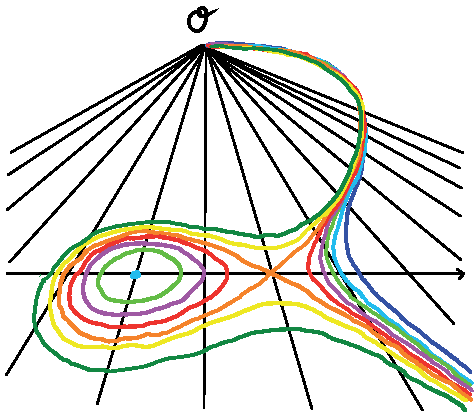
\includegraphics[scale=1]{img/bem_11_7.pdf}
		\caption{$y^2 = x^3 - 3x + s$ für \textcolor{Green4}{$s = 5$}, \ \textcolor{yellow}{$s=3$}, \ \textcolor{Orange2}{$s=2$}, \ \textcolor{red}{$s=1$}, \ \textcolor{Magenta1}{$s=0$}, \ \textcolor{green}{$s=-1$}, \ \textcolor{cyan}{$s=-1.999$}, \ \textcolor{RoyalBlue3}{$s=-5$}}
	\end{figure}
	Das Bild ist perspektivisch so verzerrt, dass der unendlich ferne Punkt $\oh$, der für die Richtung der $y$-Achse steht, am Horizont erscheint.
\end{bem}

\begin{satz}[Vereinfachte Weierstraßgleichungen]
\label{satz_11.8}
	Sei $E_F(k)$ eine elliptische Kurve mit $F$ in der langen Weierstraßform \eqref{eq_lang-weier}. \begin{enumerate}[(i)]
		\item Falls $\Char(k) \neq 2$, ist die Abbildung
		\begin{equation}
		\begin{aligned}
			\Phi \colon \PP^2(k) &\longrightarrow 2\PP^2(k) \\
			[r:s:t] &\longmapsto \benbrace*{r : s + \frac{a_1}{2}r + \frac{a_3}{2}t : t}
		\end{aligned}
		\end{equation}
		bijektiv und es ist $\Phi(E_f(k)) = E_{H_1}(k)$ ebenfalls eine elliptische Kurve mit $H_1(X,Y,Z) = Y^2Z - X^3 - \frac{1}{4}b_2 X^2Z - \frac{1}{2} b_4 XZ^2 - \frac{1}{4} b_6 Z^3$, wobei $b_2 = a_1^2 + 4a_2, b_4 = 2a_4 + a_1 a_3, b_6 = a_3^2 + 4a_6$.
		\item Falls $\Char(k) \neq 2$ und $\Char(k) \neq 3$, ist die Abbildung
		\begin{equation}
		\begin{aligned}
			\Psi\colon \PP^2(k) &\longrightarrow \PP^2(k) \\
			[r:s:t] &\longmapsto [36r + 3b_2 t : 216s : t]
		\end{aligned}
		\end{equation}
		bijektiv und es ist $\Psi(E_{H_1}(k)) = E_{H_2}(k)$ ebenfalls eine elliptische Kurve mit $H_2(X,Y,Z) = Y^2Z - X^3 + 27c_4 XZ^2 + 54 c_6 Z^3$, wobei $c_4 = b_2^2 - 24b_4, c_6 = -b_2^3 + 36b_2b_4 - 216b_6$.
	\end{enumerate}
\end{satz}

\begin{bem}
	Wir können die lange Weierstraßgleichung im Fall $\Char(k) \neq 2$ also stets zur affinen Gleichung $y_2 = x^3 + a_2x^2 + a_4 x + a_6$ vereinfachen; falls $\Char(k) \neq 2$ und $\Char(k)= \neq 3$ gilt, sogar zu $y^2 = x^3 + a_4 x + a_6$. Wir nennen diese Gleichung die \Index{kurze Weierstraßform}, das entsprechende Polynom dann das \bet{kurze Weierstraßpolynom}.
\end{bem}

\begin{bem}
	Auch im Fall $\Char(k) = 2$ lässt sich die lange Weierstraßgleichung vereinfachen, das ist nicht schwierig, wenn $a_1 \neq 0$, aber auch für $a_1 = 0$ möglich. Wir behandeln dies hier nicht näher.
\end{bem}

\begin{bew}
	Zunächst zu (i): \begin{itemize}
		\item $\Phi$ ergibt als Abbildung nur Sinn, wenn $2$ invertierbar ist in $k$, das heißt, falls $\Char(k) \neq 2$ ist. $\Phi$ ist dann bijektiv, da $\Phi$ die Umkehrabbildung $\Phi^{-1}([r:s:t]) = \benbrace*{r : s - \frac{a_1}{2}r - \frac{a_3}{2}t : t}$ hat.
		\item Weiter bezeichnen wir mit $\Phi, \Phi^{-1}$ auch die zugehörigen (affinen) Abbildungen $\Phi, \Phi^{-1}\colon k^3 \longrightarrow k$,\linebreak $\Phi(r,s,t) = \enbrace*{r,s+ \frac{a_1}{2}r + \frac{a_3}{2}t, t}$ bzw. $\Phi^{-1}(r,s,t) = \enbrace*{r,s - \frac{a_1}{2}r - \frac{a_3}{2}t,t}$. Nun können wir mit den im Satz angegebenen Zahlen $b_2,b_4,b_6$ nachrechnen, dass $H_1(X,Y,Z) = F\enbrace*{X,Y - \frac{a_1}{2}X - \frac{a_3}{2}Z,Z}$:
		\begin{equation}
		\begin{aligned}
			& \quad \ F\enbrace*{X,Y-\frac{a_1}{2}X-\frac{a_3}{2}Z,Z} \\
			&= \enbrace*{Y- \frac{a_1}{2} X - \frac{a_3}{2}Z}^2 Z + a_1 X \enbrace*{Y - \frac{a_1}{2} X - \frac{a_3}{2}Z}Z + a_3 \enbrace*{Y - \frac{a_1}{2} X - \frac{a_3}{2} Z}Z^2 \\
			& \quad \ - X^3 - a_2X^2Z - a_4 XZ^2 - a_6Z^3 \\
			&= Z \cdot \enbrace*{Y^2 - 2Y \enbrace*{\frac{a_1}{2}X + \frac{a_3}{2} Z} + \enbrace*{\frac{a_1^2}{4} X^2 + 2 \cdot \frac{a_1 a_3}{4} XZ + \frac{a_3^2}{4} Z^2}} \\
			& \quad \ + a_1XYZ - \frac{a_1^2}{2} X^2 Z - \frac{a_1 a_3}{2} XZ^2 + a_3 YZ^2 - \frac{a_1 a_3}{2} XZ^2 - \frac{a_3^2}{2} Z^3 - X^3 - a_2 X^2 Z - a_4 XZ^2 - a_6Z^3 \\
			&= Y^2 Z - X^3 + \enbrace*{-\frac{a_1^2}{4} - a_2} X^2 Z + \enbrace*{- \frac{a_1 a_3}{2} - a_4} XZ^2 + \enbrace*{- \frac{a_3^2}{4} - a_6} Z^3 \\
			&= Y^2 Z - X^3 - \frac{1}{4} b_2 X^2 Z - \frac{1}{2} b_4 XZ^2 - \frac{1}{4} b_6 Z^3 = H_1(X,Y,Z)
		\end{aligned}
		\end{equation}
		\item Es folgt $H_1(r,s,t) = F(\Phi^{-1}(r,s,t))$, also gilt $F(r,s,t) = 0$ genau dann, wenn $H_1(\Phi(r,s,t))=0$, sodass $\Phi (E_F(k)) = \cc_{H_1}(k)$ folgt. Es bleibt zu zeigen, dass $\cc_{H_1}(k)$ nicht-singulär ist: Mit der Kettenregel rechnen wir nach:
		\begin{equation}
		\begin{aligned}
			\frac{\der H_1}{\der X}(r,s,t) &= \frac{\der F}{\der X}(\Phi^{-1}(r,s,t)) - \frac{a_1}{2} \frac{\der F}{\der Y}(\Phi^{-1}(r,s,t)) \\
			\frac{\der H_1}{\der Y}(r,s,t) &= \frac{\der F}{\der Y} (\Phi^{-1}(r,s,t)) \\
			\frac{\der H_1}{\der Z}(r,s,t) &= -\frac{a_3}{2} \frac{\der F}{\der Y} \Phi^{-1}(r,s,t) + \frac{\der F}{\der Z}(\Phi^{-1}(r,s,t))
		\end{aligned}
		\end{equation}
		\item Ist $P = [r:s:t] \in \cc_{H_1}(\overline{k})$, dann ist $\Phi^{-1}(P) = \Phi^{-1}([r:s:t])$ als Punkt der Kurve $\cc_F(\overline{k})$ nicht-singulär, da $F$ elliptische Kurve ist. Die drei Ableitungen von $F$ in $\Phi^{-1}(P)$ sind also nicht alle $= 0$, also sind auch die drei Ableitungen von $H_1$ in $(r,s,t)$ nicht alle $=0$. Also ist $P$ auf $\cc_{H_1}(\overline{k})$ nicht-singulär.
	\end{itemize}
	Zu (ii): $\Psi$ hat die Inverse $[r:s:t] \mapsto \benbrace*{\frac{1}{36} r - \frac{b_2}{12}t : \frac{1}{216} s : t}$, da wegen $\Char(k) \neq 2, \neq 3$ die Zahlen $\frac{1}{36}, \frac{1}{12}, \frac{1}{216} = \frac{1}{2^3 \cdot 3^3}$ in $k$ existieren, und leicht zu bestätigen ist, dass $\Psi(\Psi^{-1}([r:s:t])) = [r:s:t]$ gilt. Durch geduldiges Nachrechnen zeigt man $H_2(X,Y,Z) = 2^6 3^6 \cdot H_1 \enbrace*{\frac{1}{36} X - \frac{b_2}{12}Z, \frac{1}{216} Y,Z}$, daraus folgt $H_1(r,s,t) = 0$ genau dann, wenn $H_2(\Psi(r,s,t))=0$, das heißt $\Psi(E_{H_1}(k)) = \cc_{H_2}(k)$. Wieder mit der Kettenregel kann auch die Nicht-Singularität von $\cc_{H_2}$ gezeigt werden. \qed
\end{bew}

Wir definieren zwei wichtige Kennzahlen projektiver Kurven wie folgt:
\begin{defn}[Diskriminante, $j$-Invariante]
	Sei $\cc_F(k)$ die projektive ebene Kurve zum langen Weierstraßpolynom \eqref{eq_lang-weier}. Dann heißt die Zahl
	\[ \Delta = \Delta(\cc_F(k)) = -b_2^2 b_8 - 8b_4^3 - 27b_6^2 + 9b_2b_4b_6 \]
	mit $b_2 = a_1^2 + 4a_2, b_4 = 2a_4 + a_1 a_3, b_6 = a_3^2 + 4a_6$ und $b_8 = a_1^2 a_6 + 4a_2 a_6 - a_1a_3a_4 + a_2 a_6^2 - a_4^2$ die \Index{Diskriminante} der Kurve $\cc_F(k)$. Die Zahl 
	\[ j = j(\cc_F(k)) := \frac{(b_2^2 - 24b_4)^3}{\Delta} = \frac{c_4^3}{\Delta} \]
	heißt die \bet{$j$-Invariante} der Kurve $\cc_F(k)$. \index{j-Invariante@$j$-Invariante}
\end{defn}

\begin{bem}
	\begin{itemize}
		\item Die $j$-Invariante legt die Isomorphieklasse der elliptischen Kurve über $\overline{k}$ fest: Zwei elliptische Kurven sind isomorph über $\overline{k}$ genau dann, wenn sie dieselbe $j$-Invariante besitzen (ohne Beweis).
		\item $j$ ist unabhängig von der Wahl der speziellen Kurvengleichung.
	\end{itemize}
\end{bem}

\begin{bem}
	Die Diskriminante einer Kurve $\cc_F(k)$ ist ein nützliches Hilfsmittel, um zu testen, ob eine Kurve, die durch eine lange Weierstraßgleichung gegeben ist, nicht-singulär (und damit elliptisch) ist:
\end{bem}

\begin{satz}
	Sei die Kurve $\cc_F(k)$ gegeben durch das lange Weierstraßpolynom $F$. Dann ist $\cc_F(k)$ nicht-singulär genau dann, wenn $\Delta(\cc_F(k)) \neq 0$ ist.
\end{satz}

Mit der angegebenen Formel für $\Delta$ ist dies auch rechnerisch leicht zu testen -- wichtig, um elliptische Kurven für die Anwendungen zu konstruieren. Dieses Diskriminantenkriterium zeigen wir im nächsten Abschnitt.
\nextlecture
\subsubsection{Das Diskriminantenkriterium}
\begin{defn}[Diskriminante]
	Sei $\cc_F(k)$ die projektive ebene Kurve zum langen Weierstraßpolynom \marginnote{[12]}
	\[ F(X,Y,Z) = Y^2Z + a_1XYZ + a_3YZ^2 - X^3 - a_2X^2Z - a_4 XZ^2 - a_6Z^3. \]
	Dann heißt die Zahl
	\[ \Delta = \Delta(\cc_F(k)) = -b_2^2 b_8 - 8b_4^3 - 27b_6^2 + 9b_2b_4b_6 \]
	mit $b_2 = a_1^2 + 4a_2, b_4 = 2a_4+a_1a_3, b_6 = a_3^2+4a_6$ und $b_8 = a_1^2 a_6 + 4a_2a_6-a_1a_3a_4 + a_2a_3^2 - a_4^2$ die \Index{Diskriminante} der Kurve $\cc_F(k)$.
\end{defn}

\begin{bem}
	Im Fall einer Kurve $\cc_F(k)$ in einer kurzen Weierstraßform $f(x,y) = y^2-x^3-ax-b$ haben wir $\Delta(\cc_F(k)) = -8 \cdot (2a)^3 - 27 \cdot (4b)^2 = -16 \cdot (4a^3 + 27b^2)$, da $a_1 = 0, a_3 = 0, a_2 = 0, a_4 = a, a_6 = b$, also $b_2 = 0, b_4 = 2a, b_6 = 4b, b_8 = -a^2$. (vgl. Übungsaufgabe 3 auf Blatt 4).
\end{bem}

Wir zeigen das Diskriminantenkriterium:
\begin{satz}[Diskriminantenkriterium]
\label{satz_12.3}
	Sei die Kurve $\cc_F(k)$ gegeben durch das lange Weierstraßpolynom $F$. Dann ist $\cc_F(k)$ nicht-singulär genau dann, wenn $\Delta(\cc_F(k)) \neq 0$ ist.
\end{satz}

\begin{bem}
	\begin{itemize}
		\item Bei diesem Kriterium, wenn $\Delta \neq 0$, erhalten wir, dass $\cc_F(\overline{k})$ über dem algebraischen Abschluss $\overline{k}$ keine singulären Punkte enthält (insbesondere auch über $k$, aber über $\overline{k}$ ist eben noch stärker). Deswegen haben wir uns bei unserer Definition von "nicht-singuläre Kurve" auf $\overline{k}$ bezogen, was wegen Satz~\ref{satz_12.3} also mathematisch leichter wird. Für $\Char(k) \neq 2$ kann es aber nicht sein, dass $\cc_F$ über $k$ keine singulären Punkte hat und über $\overline{k}$ hingegen schon.
		\item Das Kriterium ist in der Praxis nützlich, da eine Kurve in Weierstraßform (die vielleicht per Zufallsgenerator für die Koeffizienten erzeugt worden ist), damit leicht auf Nicht-Singularität durch Berechnung der einfachen Formel für $\Delta$ getestet/überprüft werden kann.
		\item Der Beweis unterscheidet wesentlich die Fälle $\Char(k) = 2, \Char(k) = 3$ und sonst.
	\end{itemize}
\end{bem}

\begin{bew}
	Die Kurve $\cc_F(k)$ ist nicht-singulär genau dann, wenn ihre affine Kurve $\cc_F(k)$ mit $f(x,y) = y^2 + a_1xy + a_3y - x^3 - a_2x^2 - a_4 x - a_6$ nicht-singulär ist. Wir zeigen den Satz deswegen im Affinen (der einzige nicht-affine Punkt $\oh = [0:1:0]$ der Kurve ist immer regulär, vgl. Bemerkung~\ref{bem_11.5}). Nun enthält $\cc_F(\overline{k})$ einen singulären Punkt $(r,s)$ genau dann, wenn
	\[ f(r,s) = 0 \qquad \underbrace{\frac{\der f}{\der x} (r,s)}_{a_1 s - 3r^2 - 2a_2r - a_4} = 0 \qquad \underbrace{\frac{\der f}{\der y} (r,s)}_{=2s + a_1 r + a_3} = 0 \]
	gilt. Wir unterscheiden weiter mehrere Fälle nach dem Wert der Charakteristik von $k$.
\end{bew}

\begin{bew}[1. Fall: $\Char(k)= 2$ und $a_1 = 0$]
	\begin{description}
		\item["$\Leftarrow$":] Dann ist hier $b_2 = b_4 = 0, b_6 = a_3^2, \Delta = -27a_3^4 = a_3^4$. Weiter gilt $\frac{\der f}{\der y} = a_3$, sodass, falls ein singulärer Punkt existiert, dann $a_3 = 0$ und $\Delta = 0$ folgt.
		\item["$\Rightarrow$":] Ist $\Delta = 0$, folgt $\frac{\der f}{\der y} = 0$. Nun existieren $r,s \in \overline{k}$ mit $r^2 + a_4=0, s^2 + a_3s = r^3 + a_2r^2 + a_4r + a_6$, also ist $(r,s) \in \aff^2(\overline{k})$ singulärer Punkt auf $\cc_f(\overline{k})$.
	\end{description}
\end{bew}

\begin{bew}[2. Fall: $\Char(k) = 2$ und $a_1 \neq 0$]
	In Charakteristik $2$ gilt:
	\begin{equation}
	\begin{aligned}
		\Delta &= -a_4^4 (a_1^2 a_6 - a_1 a_3 a_4 + a_2 a_3^2 - a_4^2) - 27a_3^4 + a_1^3 a_3^3 \\
		&= a_1^6 a_6 + a_1^5 a_3a_4 + a_1^4a_2a_3^2 + a_1^4a_4^2 + a_1^3 a_3^3 +a_3^4.
	\end{aligned}
	\end{equation}
	\begin{description}
		\item["$\Leftarrow$":] Hat $\cc_f(\overline{k})$ einen singulären Punkt $(r,s)$, so ist $f(r,s) = 0$, das heißt $a_1 s + r^2 + a_4 = 0$ und $a_1 r + a_3 = 0$. Da $a_1 \neq 0$, folgt $r = \frac{a_3}{a_1}$ und $s = \frac{a_3^2+a_1^2a_4}{a_1^3}$. Durch einsetzen in $f(r,s)$ folgt $0 = f(r,s) = \Delta a_1^{-6}$, also $\Delta = 0$.		
		\item["$\Rightarrow$":] Ist $\Delta = 0$, definieren wir $r,s$ wie oben, dann ist $f(r,s) = \Delta a_1^{-6}$, also $f(r,s) = 0$, womit ein singulärer Punkt konstruiert ist.
	\end{description}
\end{bew}

\begin{bew}[3. Fall: $\Char(k)=3$]
	Via Rechnen in Charakteristik $3$ folgt $\Delta = -b_2^2 b_8 - 8b_4^3$. Betrachte die Abbildung $\Phi\colon \cc_F(k) \rightarrow \cc_{H_1}(k)$ aus Satz~\ref{satz_11.8}(i), die die lange Weierstraßform $F$ auf die kurze Form $H_1$ bringt. Es ist $\Delta(\cc_{H_1}(k)) = \Delta(\cc_F(k))$ durch Nachrechnen, somit genügt es ohne Einschränkung, das Diskriminantenkriterium für die kurze Form $H_1$ zu zeigen.
\end{bew}

\begin{bew}[Fortsetzung 3. Fall]
	Die Kurve $\cc_{H_1}(\overline{k})$ enthält genau dann einen singulären Punkt, wenn es $r,s \in \overline{k}$ gibt mit
	\[ s^2 - r^3 - \frac{1}{4} b_2 r^2 - \frac{1}{2}b_4 r - \frac{1}{4} b_6 = 0, \qquad 3r^2 + \frac{1}{2} b_2r + \frac{1}{2} b_4 = 0,  \qquad 2s = 0, \]
	das heißt falls $r$ eine doppelte Nullstelle des Polynoms $\sigma(x) := x^3 + \frac{1}{4} b_2 x^2 + \frac{1}{2} b_4x \frac{1}{4} b_6$ ist, sprich $\sigma(r) = 0 = \sigma'(r)$ ist. \\
	Über $\overline{k}$ zerfällt $\sigma$ in drei Linearfaktoren $\sigma(x) = (x-\alpha_1)(x-\alpha_2)(x-\alpha_3)$ mit $\alpha_i \in \overline{k}$. Nun hat ein Polynom $\sigma$ genau dann eine doppelte Nullstelle, falls seine Diskriminante $\disc(\sigma) := (\alpha_1 - \alpha_2)^2 (\alpha_1 - \alpha_3)^2 (\alpha_2 - \alpha_3)^2$ verschwindet, vgl. Bemerkung~\ref{bem_12.14}.
\end{bew}

\begin{bew}[Fortsetzung]
	Somit ist im dritten Fall zu zeigen: $\Delta = 0 \Leftrightarrow \disc(\sigma)=0$. \\
	Wegen $\disc(x^3 + ux^2 + vx + w) = u^2v^2 - 4u^3w - 4v^3 - 27w^2 + 18uvw$, vgl. Korollar~\ref{kor_12.16}, erhalten wir mit $u = \frac{b_2}{4}, v = \frac{b_4}{2}, w= \frac{b_6}{4}$ dann in Charakteristik $3$, dass $\disc(\sigma) = \frac{1}{64} b_2^2 b_4^2 - \frac{1}{64} b_2^3 b_6 - \frac{1}{2} b_4^3$. Wegen $4 b_8 = b_2 b_6 - b_4^2$ erhalten wir $\disc(\sigma) = \frac{1}{16} (-b_2^2b_8 - 8b_4^3) = \frac{1}{16} \Delta$. Aus dieser Formel folgt die Behauptung im dritten Fall.
\end{bew}

\begin{bew}[4. Fall: $\Char(k) > 3$ oder $\Char(k) = 0$]
	Mit der Bijektion $\Psi \circ \Phi \colon \cc_F(k) \rightarrow \cc_{H_2}(k)$ zum kurzen Weierstraßpolynom $H_2$ (Satz~\ref{satz_11.8}(ii)) bzw. $h_2(x,y) = y^2 - x^3 + 27c_4x + 54c_6$ mit $c_4 = b_2^2 - 24b_4, c_6 = -b_2^3 + 36b_2 b_4 - 216 b_6$, folgt durch Untersuchung der Ableitungen wieder $\cc_F(k)$ nicht-singulär genau dann, wenn $\cc_{H_2}(k)$ nicht-singulär. Wir berechnen $\Delta(\cc_{H_2}(k)) = 2^6 3^9 \cdot (c_4^3-c_6^2) = \dots = 2^{12} 3^{12} \Delta(\cc_F(k))$, also genügt es, die Behauptung für $\cc_{H_2}(k)$ zu zeigen. Wie im dritten Fall haben wir:
	\[ \cc_{H_2}(\overline{k}) \text{ enthält singulären Punkt } \quad \Leftrightarrow \quad \sigma(x) = x^3 \underbrace{- 27c_4}_{v} x \underbrace{- 54 c_6}_{w} \text{ hat doppelte Nullstelle } \quad \Leftrightarrow \quad \disc(\sigma)=0 \]
	Wegen der Formel in Korollar~\ref{kor_12.16} für $\disc(\sigma)$ folgt mit $u = 0, v = -27c_4, w= - 54c_6$:
	\[ \disc(\sigma) = 0 \quad \Leftrightarrow \quad 4 \cdot 27^3 c_4^3 - 27 \cdot 54^2 c_6^2 = 0 \quad \Leftrightarrow \quad c_4^3 - c_6^2 = 0. \]
	Daraus folgt die Behauptung. \qed
\end{bew}

Theoretische Ergänzungen zu unserer Definition von $\Delta(\cc_F(k))$:
\begin{defn}[Diskriminante eines Polynoms]
	Die \bet{Diskriminante eines Polynoms} $\sigma \in k[x], n := \deg(\sigma) \geq 1$, ist \index{Diskriminante!eines Polynoms}
	\[ \disc(\sigma) := \prod_{1 \leq i < j \leq n} (\alpha_i - \alpha_j)^2 = (-1)^{\frac{n(n-1)}{2}} \prod_{i \neq j} (\alpha_i - \alpha_j) \in \overline{k},\]
	falls $\alpha_1, \dots, \alpha_n \in \overline{k}$ die Nullstellen von $\sigma \in \overline{k}$ bezeichnen.
\end{defn}

\begin{bem}
	Man vergleiche dies mit der Diskriminante $\disc(\sigma) = p^2-4q$ eines quadratischen Polynoms $\sigma(x) = x^2+px+q \in k[x]$, wir haben $\alpha_{1,2} = -\frac{p}{2} \pm \sqrt{\frac{p^2}{4} - q} = -\frac{p}{2} \pm \frac{1}{2} \sqrt{p^2 -4q}$, also genau $(\alpha_1 - \alpha_2)^2 = \disc(\sigma)$. Ist dies $=0$, ist $\alpha_1 = \alpha_2$ eine doppelte Nullstelle von $\sigma$.
\end{bem}

\begin{bem}
\label{bem_12.14}
	$\disc(\sigma)$ verschwindet genau dann, wenn $\sigma$ über $\overline{k}$ eine doppelte Nullstelle hat. Dies folgt unmittelbar aus der Definition von $\sigma$.
\end{bem}

\begin{bem}
\label{bem_12.15}
	\begin{itemize}
		\item Ist $\sigma \in k[x], n = \deg(\sigma) \geq 1$, ein normiertes Polynom, kann die Beziehung $\disc(\sigma) = (-1)^{n(n-1)/2} \cdot \Res(\sigma, \sigma')$ mit der in Definition~\ref{def_10.5} behandelten Resultante gezeigt werden.
		\item Aus dieser wichtigen Formel folgt wegen unserer Definition für die Resultante, dass stets $\disc(\sigma) = k$ gilt.
	\end{itemize}
\end{bem}

\begin{kor}
\label{kor_12.16}
	Es gilt $\disc(x^3+ux^2+vx+w) = u^2v^2 - 4wu^3 - 4v^3 - 27w^2 + 18uvw$. 
\end{kor}

\minisec{Beweis}
	Für $\sigma(x) = x^3 + ux^2 + vx + w$ und $\sigma'(x) = 3x^2+2ux+v$ ist nach Defintion~\ref{def_10.5}: \marginnote{Genaue Rechnung im Skript!}
	\[ M(\sigma,\sigma') = \begin{pmatrix}
	w & 0 & v & 0 & 0 \\ 
	v & w & 2u & v & 0 \\ 
	u & v & 3 & 2u & v \\ 
	1 & u & 0 & 3 & 2u \\ 
	0 & 1 & 0 & 0 & 3
	\end{pmatrix} \]
	Durch Berechnung von $\Res(\sigma) = \det(M(\sigma,\sigma'))$ und $(-1)^{3 \cdot (3-1)/2} = -1$ folgt die Behauptung. \qed
	
\nextlecture
\subsubsection{Die Gruppenstruktur elliptischer Kurven}
	Sei $E(k)$ eine elliptische Kurve über einem Körper $k$. \marginnote{[13]}
	
\begin{satz}
\label{satz_13.1}
	\begin{enumerate}[(a)]
		\item Seien $P,Q \in E(k), P \neq Q$, und $G=G(P,Q) \subseteq \PP^2(k)$ die projektive Gerade, die $P$ und $Q$ verbindet. Dann hat $G$ noch einen dritten Schnittpunkt mit $E(k)$ gemäß Vielfachheiten gezählt (das heißt, eventuell $P$ bzw. $Q$ selbst, falls $m(P;G,E(k)) = 2$ bzw. $m(Q;G,E(k)) = 2$).
		\item Sei $G$ die Tangente an $E(k)$ im Punkt $P \in E(k)$. Dann hat $G$ noch einen dritten Schnittpunkt mit $E(k)$ gemäß der Vielfachheiten gezählt (das heißt, eventuell $P$ selbst, falls $m(P;G,E(k)) = 3$).
	\end{enumerate}
\end{satz}

\begin{bew}
	Als Ergänzung zum Satz von Bézout haben wir Satz~\ref{satz_10.15} kennen gelernt, der im Spezialfall $\deg(F_1) = 1,\linebreak \deg(F_2) = 3$ dann $\sum_{P \in \cc_{F_1} \cap \cc_{F_2}} m(P;\cc_{F_1},\cc_{F_2}) \in \{0,1,3\}$ liefert (siehe Beispiel~\ref{bsp_10.16}). Also gilt auch hier: \linebreak $\sum_{R \in G \cap E(k)} m(R;G,E(k)) \in \{0,1,3\}$.
	\begin{description}
		\item[zu (a):] Ist $G = G(P,Q)$, folgt $2 \leq  \#(G \cap E(k)) \leq \sum_{R \in G \cap E(k)} m(R;G,E(k)) \in \{0,1,3\}$. Das geht nur, wenn die Vielfachensumme $3$ ist, also existiert ein $R \in G \cap E(k)$ \begin{itemize}
			\item mit $R \notin \{P,Q\}$, falls $m(P;G,E(k)) = 1 = m(Q;G,E(k))$,
			\item oder mit $R = P$, falls $m(P;G,E(k)) = 2$
			\item oder mit $R = Q$, falls $m(Q;G,E(k)) = 2$.
		\end{itemize} 
		\item[zu (b):] Ist $G$ die Tangente an $E(k)$ in $P \in E(k)$, ist $m(P;G,E(k)) \geq 2$ nach Satz~\ref{satz_9.22}. Es folgt wie im Beweis zu (a) wieder, dass die Vielfachensumme $3$ ist, also die Existenz eines $R \in G \cap E(k)$ mit $R \neq P$, falls $m(P;G,E(k)) = 2$ und $R = P$, falls $m(P;G,E(k)) = 3$ gilt. \qed
	\end{description}
\end{bew}

\begin{bsp}
	Betrachte die elliptische Kurve $E(k)$ zur (kurzen) Weierstraßgleichung $y^2 = x^3 - 3x + 3$. Jede Gerade, die $E(k)$ in zwei Punkten schneidet, schneidet $E(k)$ in einem dritten Punkt, gemäß Vielfachheit gezählt. Der dritte Schnittpunkt kann auch $\oh \in g_\infty$ sein. \todo{Bild texen!}
	\newpage
	\begin{figure}[h]
		\centering
		\begin{tikzpicture}[scale=1]
			\draw [thick,samples=500,smooth,domain=-2.10378:2.4,variable=\x,blue] plot ({\x},{(\x*\x*\x-3*\x+3)^(0.5)});
			\draw [thick,smooth,domain=-2.10378:2.4,variable=\x,blue] plot ({\x},{-(\x*\x*\x-3*\x+3)^(0.5)});
			
			\draw (-2.1038,0) node[fill,circle,inner sep=2pt,red]{};
			\draw (-2.2,0) node[align=right,anchor=east]{$S$};
			\draw [very thick](-2.1038,-2.5) -- (-2.1038,2.5);
			
			\draw (.292037,-1.46588) node[fill,circle,inner sep=2pt,red]{};
			\draw (.292037,-1.46588) node[align=left,anchor=north west]{$W$};
			\draw [very thick,smooth,domain=-.7:1.3,variable=\x] plot ({\x},{.936007*\x-1.73923});
			
			\draw (1.8,-1.85257) node[fill,circle,inner sep=2pt,red]{};
			\draw (1.8,-1.85257) node[align=left,anchor=south west]{$U$};
			\draw (-.31049,1.97523) node[fill,circle,inner sep=2pt,red]{};
			\draw (-.31049,1.97523) node[align=left,anchor=south west]{$U*U$};
			\draw [very thick,smooth,domain=-.7:2.2,variable=\x] plot ({\x},{-1.8137*\x+1.4121});
			
			\draw (-1.8,-1.6025) node[fill,circle,inner sep=2pt,red]{};
			\draw (-1.8,-1.6025) node[align=left,anchor=north,yshift=-.2cm]{$P$};
			\draw (.8,1.05451) node[fill,circle,inner sep=2pt,red]{};
			\draw (.8,1.05451) node[align=left,anchor=north west]{$Q$};
			\draw (2.044337,2.32614) node[fill,circle,inner sep=2pt,red]{};
			\draw (2.044337,2.32614) node[align=left,anchor=north west]{$P*Q$};	
			\draw [very thick,smooth,domain=-2.5:2.5,variable=\x] plot ({\x},{1.02193*\x+0.236968});
		\end{tikzpicture}
		\caption{Veranschaulichung der Definition~\ref{def_13.4} an dem Beispiel $y^2=x^3-3x+3$: Für zwei verschiedene Punkte $P,Q$ definieren wir $P*Q$ als den dritten Schnittpunkt der Gerade durch $P$ und $Q$. Das kann wieder $P$ oder $Q$ sein, falls die Gerade eine Tangente durch $P$ oder $Q$ ist. Für einen Punkt $U$ setzen wir $U * U$ als den weiteren Schnittpunkt der Tangente durch $U$; dieser kann auch $\oh$ sein (z.B. im Fall von $S$). Ein Wendepunkt $W$ ist bereits dreifacher Schnittpunkt, daher definieren wir hier $W * W = W$.}
	\end{figure}
\end{bsp}

Wir möchten auf $E(k)$ eine Verknüpfung "$+$" erklären, also eine Punkteaddition $P + Q$, bei der wiederum ein Punkt auf der elliptischen Kurve herauskommt. Den dritten Schnittpunkt, den die Gerade $G(P,Q)$ durch zwei Punkte $P$ und $Q$ auf $E(k)$ mit $E(k)$ hat laut Satz~\ref{satz_13.1}, bezeichnen wir mit $P * Q$.

\begin{defn}[dritter Schnittpunkt]
\label{def_13.4}
	Für $P,Q \in E(k)$, $P \neq Q$ definieren wir also:
	\[ P * Q := \begin{cases}
		R \in (G(P,Q) \cap E(k)) \setminus \{P,Q\}, & \text{falls } m(P;G,E(k)) = 1 = m(Q;G,E(k)) \\
		P, & \text{falls } m(P;G,E(k)) = 2 \\
		Q, & \text{falls } m(Q;G,E(k)) = 2,
	\end{cases} \]
	sowie
	\[ P * P := \begin{cases}
		R \in (T_P(E(k)) \cap E(k)) \setminus \{P\}, & \text{falls } m(P;T_p(E(k)),E(k)) = 2 \\
		P, & \text{falls } m(P;T_P(E(k)),E(k)) = 3 \text{ (d.h. falls } P \text{ Wendepunkt)}
	\end{cases} \]
\end{defn}

\begin{bem}
	\begin{itemize}
		\item Der unendlich ferne Punkt $\oh \in E(k)$ erfüllt $\oh * \oh = \oh$, da er ein Wendepunkt ist.
		\item Weiter ist offensichtlich $P * Q = Q * P$ aufgrund der Definition.
		\item Es gilt: $R = P * Q \Rightarrow P = Q * R \Rightarrow Q = R * P$, das heißt $P * (P * Q) = Q$ für alle $P,Q \in E(k)$. \hfill [\#]
		\item Damit gilt auch $P * Q = P * R \Leftrightarrow Q = R$, denn $P * Q = P * R \Rightarrow P*(P*Q)=P*(P*R) \Rightarrow Q=R$.
	\end{itemize}
\end{bem}

\begin{bem}
	Man beachte, dass für $P = [a:b:1] \in \PP^2(k) \cap \iota(\aff^2(k))$ die Gerade $G(P,Q) = G(c,0,-a) = \{ [x:y:z] \in \PP^2(k) : x - az = 0\}$ im Affinen eine Parallele zur $y$-Achse darstellt (Gleichung $x = a$). Für eine elliptische Kurve, die durch eine kurze Weierstraßform gegeben und (für $\Char(k) \neq 2$) symmetrisch zur $x$-Achse ist, wird typischerweise $P * \oh \neq P$ sein. Wegen $(\oh * \oh) * P = \oh * P$ einerseits, da $\oh * \oh = \oh$, und $\oh * (\oh * P) = P$ andererseits wegen [\#], kann die Verknüpfung $*$ also nicht assoziativ sein. Stattdessen setzen wir unsere Verknüpfung "$+$" wie folgt:
\end{bem}

\begin{defn}[Punkteaddition auf elliptischen Kurven]
	Für $P,Q \in E(k)$ definieren wir
	\[P + Q := \oh *(P * Q). \]
	Ist $E(k)$ in kurzer Weierstraßform und (für $\Char(k) \neq 2$) symmetrisch zur $x$-Achse, erhält man $P+Q$, indem man den dritten Schnittpunkt $P*Q$ von $G(P,Q)$ mit $E(k)$ dann noch an der $x$-Achse spiegelt, das heißt das Negative des $y$-Wertes nimmt.
\end{defn}

\begin{bem}
\label{bem_13.8}
	\begin{itemize}
		\item Es gilt $\oh + P = \oh * (\oh * P) = P$ nach [\#], das heißt $\oh$ ist neutrales Element bezüglich $+$.
		\item Es gilt $-P = \oh * P$, da $P + (\oh * P) = \oh * (P * (\oh * P)) = (P * (\oh * P)) * \oh = (P * (P * \oh)) * \oh = \oh$ nach [\#].
	\end{itemize}
\end{bem}
Es ist nicht auf Anhieb zu sehen, dass hier mit "$+$" eine elliptische Kurve $E(k)$ zu einer Gruppe $(E(k),+)$ wird, sprich, ob das Assoziativgesetz gilt.

\begin{lemma}
\label{lemma_13.9}
	Liegen drei Punkte $P,Q,R \in E(k)$ einer elliptischen Kurve auf einer projektiven Gerade $G$, so gilt $(P+Q) + R = \oh$ und umgekehrt. Dabei müssen $P,Q,R$ nicht notwendig verschieden sein.
\end{lemma}

\minisec{Beweis}
	Da $R = P *Q$ nach Voraussetzung, folgt $-R = \oh * R = \oh * (P * Q) = P+Q$. Umgekehrt gilt das ebenso. \qed
	
\begin{satz}[Elliptische Kurve mit Punktaddition ist abelsche Gruppe, Poincaré, 1901]
	Sei $k$ ein beliebiger Körper und $E(k)$ eine elliptische Kurve. Die Verknüpfung $+ \colon (P,Q) \mapsto P +Q$ macht $E(k)$ zu einer abelschen Gruppe $(E(k),+)$ mit neutralem Element $\oh$, das heißt:
	\begin{enumerate}[(i)]
		\item $P+\oh = P$ für alle $P \in E(k)$.
		\item Für alle $P \in E(k)$ existiert ein $Q \in E(k)$ mit $P+Q = \oh$; setze $-P := Q$.
		\item $P + Q = Q + P$ für alle $P,Q \in E(k)$.
		\item $(P+Q) + R = P+(Q+R)$ für alle $P,Q,R \in E(k)$.
	\end{enumerate}
\end{satz}

\minisec{Beweis}
	\begin{enumerate}[(i)]
		\item Siehe Bemerkung~\ref{bem_13.8}.
		\item Für $P \in E(k)$ setze $Q := \oh * P$, siehe Bemerkung~\ref{bem_13.8}.
		\item Klar aufgrund der Definition von $P+Q$.
		\item Beweis folgt im nächsten Vorlesungsteil. \qed
	\end{enumerate}
	
\begin{bem}
	\begin{itemize}
		\item Anstelle von $\oh$ könnte man prinzipiell jeden Punkt $Q \in E(k)$ zum neutralen Element von $+$ machen, indem man $U \oplus V := U + V - Q$ setzt: Dann ist $U \oplus Q = U + Q - Q = U, U \oplus(-U+2Q) = U-U+2Q-Q = Q$ und $(U \oplus V) \oplus W = U + V + W - 2Q = U \oplus (V \oplus W)$. Die Eigenschaft von Lemma~\ref{lemma_13.9} gilt immer noch, wenn für $Q$ ein Wendepunkt genommen wird. Nun kann eine elliptische Kurve bis zu neun Wendepunkte haben, vergleiche Übungsaufgabe 4 (a) auf Blatt 5.
		\item Die Wahl von $\oh := [0:1:0]$ als Wendepunkt von $E(k)$, das heißt mit $\oh * \oh = \oh$, hat den Vorteil, dass die explizite Formel für $+$ rechnerisch einfacher wird, weil dann die Gleichung von $E(k)$ in einfacher (langer oder kurzer) Weierstraßform vorliegt. Diese Formel wird in Satz~\ref{satz_13.13} bzw. Satz~\ref{satz_13.14} angegeben.
		\item Invertieren, das heißt Berechnen von $-P = P * \oh$, ist dann bei kurzer Weierstraßform in $\Char(k) \neq 2$ und $\Char(k) \neq 3$ besonders leicht: Man spiegelt $P$ an der $x$-Achse und erhält $-P$, das heißt ist $P = [a:b:c]$, gilt $-P = [a:-b:c]$. Schnittpunkte von $E(k)$ mit der $x$-Achse sind dann selbstinvers, das heißt für $P = [a:0:c] \in E(k)$ gilt $-P = P$.
	\end{itemize}
\end{bem}

\begin{bsp}
	Betrachte $E(\RR)$ mit der Gleichung $y^2 = x^3 + 17$ bzw. $Y^2Z = X^3 + 17Z^3$. Dann liegen $P = [-1:4:1]$ und $Q = [-2:3:1]$ auf der Kurve. Ihre Verbindungsgerade ist $G(P,Q) = \{ [x:y:z] \in \PP^2(\RR) : x-y+5z = 0\}$. Um $P+Q$ zu berechnen, bestimmen wir den dritten Schnittpunkt $P*Q$ von $G(P,Q)$ und $E(\RR)$ wie folgt: Setze $y = x + 5$ ein und erhalte $(x+5)^2 = x^3 + 17 \Leftrightarrow x^3 - x^2 - 10x - 8 = 0$. Da $x = -1, x = -2$ Nullstelle der linken Seite sind, führt Polynomdivision durch $(x+1)(x+2)$ zu $x^3-x^2-10x-8 = (x+1)(x+2)(x-4)$. Der Punkt $P * Q$ hat also die $x$-Koordinate $4$; da er auf $G$ liegt, folgt $P*Q = [4:9:1]$. Es folgt $P + Q = [4:-9:1]$.
\end{bsp}

Ist $E(k)$ gegeben durch das lange Weierstraßpolynom
\[ F(X,Y,Z) = Y^2Z + a_1 XYZ + a_3 YZ^2 - X^3 - a_2X^2Z - a_4 XZ^2 - a_6 Z^3 \]
bzw. $f(x,y) = y^2 + a_1xy + a_3y - x^3 - a_2x^2 - a_4x - a_6$, so möchten wir die Addition "$+$" für die Krypto-Anwendungen in einer expliziten Formel beschreiben:

\begin{satz}[Punkteaddition bei langer Weierstraßform]
\label{satz_13.13}
	Sei $E(k)$ gegeben durch das lange Weierstraßpolynom $F$. Dann gilt: \begin{enumerate}[(a)]
		\item $P = (u,v) \in E(k) \cap \aff^2(k) \Rightarrow -P = (u,-v-a_1u-a_3)$
		\item Sei $P = (u,v), Q = (r,s) \in E(k) \cap \aff^2(k)$. \begin{itemize}
			\item Ist $u = r$ und $v + s + a_1 u + a_3 = 0$, gilt $P + Q = \oh$.
			\item Sonst ist \marginnote{Beweis wäre langweiliges Nachrechnen\dots}
			\[ P + Q = (\underbrace{\lambda^2 + a_1 \lambda - a_2 - u - r}_{=:x_3}, -(\lambda + a_1) x_3 - \mu - a_3), \] wobei
			\[ \lambda = \frac{s-v}{r-u}, \quad \mu = \frac{vr - su}{r-u}, \quad \text{ falls } r \neq u, \]
			und
			\[ \lambda = \frac{3u^2 + 2a_2 u +a_4 - a_1 v}{2v + a_1u + a_3}, \quad  \mu = \frac{-u^3 + a_4 u + 2a_6 - a_3v}{2v + a_1u + a_3}, \quad \text{ falls } r = u. \]
		\end{itemize}
	\end{enumerate}
\end{satz}

Wir geben den Beweis für die Formel bei kurzer Weierstraßform, wo er leicht zu machen ist:
\begin{satz}[Punkteaddition bei kurzer Weierstraßform]
\label{satz_13.14}
	Ist $E(k)$ gegeben durch $f(x,y) = y^2 - x^3 - ax - b$, so gilt:
	\begin{enumerate}[(a)]
		\item Für $P = (u,v) \in E(k)$ gilt $-P = (u,-v)$.
		\item Für $P = (u,v), Q = (r,s)$ mit $P \neq -Q$ ist
		\[ P + Q = (\underbrace{\lambda^2 - u - r}_{=:x}, \lambda(u-x) - v), \]
		wobei
		\[ \lambda = \begin{cases}
			\frac{s-v}{r-u}, & \text{falls } P \neq Q \\
			\frac{3u^2+a}{2v}, & \text{falls } P = Q.
		\end{cases} \]
	\end{enumerate}
\end{satz}

\minisec{Beweis}
	(a) ist klar. Zu (b): Sei $P \neq \pm Q$. Haben $g(P,Q) = \{ (u+t,v + \lambda t) : t \in \RR\}$ mit $\lambda := \frac{s-v}{r-u}$, sowie $f(u+t, v+ \lambda t) = (v + \lambda t)^2 - (u+t)^3 - a(u+t) - b$ mit den Nullstellen $t = 0, t = r-u$. Eine weitere Nullstelle ist $t = x-u$. Die Nullstellensumme $0 + r-u + x - u = r + x - 2u$ ergibt den Koeffizienten vor $t^2$ des Polynoms, nämlich $\lambda^2 - 3u$; es folgt $x = \lambda^2 - u - r$. Die $y$-Koordinate des Punkts auf $g(P,Q)$ ist dann $v + \lambda(x - u)$, für $P+Q$ dann das Negative. \\
	Ist $Q = P, P \neq -P$ (das heißt $v \neq 0$), nimmt man die Tangente an $E(k)$ im Punkt $P$, also
	\begin{equation}
	\begin{aligned}
		t_P(E(k)) &= \{(x,y) : (-3u^2 - a)x + 2vy + v^2 - 2au - 3b = 0\} \\
		&= \{ (u+t, v+ \lambda t) : t \in \RR\}
	\end{aligned}
	\end{equation}
	mit der Steigung $\lambda := \frac{3u^2 + a}{2v}$. Der Rest der Rechnung geht wie eben; es folgt $x = \lambda^2$ (da $u=r$) und der angegebene $y$-Wert für $P+P$. \qed

%\appendix							% Anhang beginnt hier (Nummerierung mit Buchstaben)
\printindex							% Index ausgeben
\subsection*{Liste der Sätze und Definitionen}
\listtheorems{satz,defn,lemma}					% listet angegebene Sätze mit Namen und Seitenzahl auf
\end{document}